\documentclass[12pt, titlepage]{article}
\usepackage{pdflscape}
\usepackage{longtable}
\usepackage{booktabs}
\usepackage{tabularx}
\usepackage{hyperref}
\usepackage{siunitx}
\usepackage{booktabs}
\usepackage{graphicx}
\usepackage[margin=1in]{geometry}
\usepackage[table]{xcolor}
\usepackage{float}
\hypersetup{
    colorlinks=true,    % Activate colored links
    linkcolor=red,      % Color of internal links
    citecolor=blue,     % Color of citation links
    urlcolor=blue,      % Color of URL links
    filecolor=black     % Color of file links
}
\usepackage[round]{natbib}

%% Comments

\usepackage{color}

\newif\ifcomments\commentstrue %displays comments
%\newif\ifcomments\commentsfalse %so that comments do not display

\ifcomments
\newcommand{\authornote}[3]{\textcolor{#1}{[#3 ---#2]}}
\newcommand{\todo}[1]{\textcolor{red}{[TODO: #1]}}
\else
\newcommand{\authornote}[3]{}
\newcommand{\todo}[1]{}
\fi

\newcommand{\wss}[1]{\authornote{blue}{SS}{#1}} 
\newcommand{\plt}[1]{\authornote{magenta}{TPLT}{#1}} %For explanation of the template
\newcommand{\an}[1]{\authornote{cyan}{Author}{#1}}

%% Common Parts

\newcommand{\progname}{ProgName} % PUT YOUR PROGRAM NAME HERE
\newcommand{\authname}{Team \#, Team Name
\\ Student 1 name
\\ Student 2 name
\\ Student 3 name
\\ Student 4 name} % AUTHOR NAMES                  

\usepackage{hyperref}
    \hypersetup{colorlinks=true, linkcolor=blue, citecolor=blue, filecolor=blue,
                urlcolor=blue, unicode=false}
    \urlstyle{same}
                                

The purpose of reflection questions is to give you a chance to assess your own
learning and that of your group as a whole, and to find ways to improve in the
future. Reflection is an important part of the learning process.  Reflection is
also an essential component of a successful software development process.  

Reflections are most interesting and useful when they're honest, even if the
stories they tell are imperfect. You will be marked based on your depth of
thought and analysis, and not based on the content of the reflections
themselves. Thus, for full marks we encourage you to answer openly and honestly
and to avoid simply writing ``what you think the evaluator wants to hear.''

Please answer the following questions.  Some questions can be answered on the
team level, but where appropriate, each team member should write their own
response:


\begin{document}

\title{Verification and Validation Report: \progname} 
\author{\authname}
\date{\today}
	
\maketitle

\pagenumbering{roman}

\section{Revision History}

\begin{tabularx}{\textwidth}{p{3cm}p{2cm}X}
\toprule {\bf Date} & {\bf Version} & {\bf Notes}\\
\midrule
March 01 & 1.0 & Nanthan completed section 3\\
March 02 & 1.1 & Kelly completed section 4\\
March 05 & 1.2 & Patrick completed section 2, 5\\
March 05 & 1.3 & Ayman completed section 7\\
March 10 & 1.4 & Reza revised all sections and added section 6,8,9,10,11\\
\bottomrule
\end{tabularx}

~\newpage

\section{Symbols, Abbreviations, and Acronyms}
This section records information for easy reference and aims to reduce ambiguity in understanding key concepts used in the project.

\subsection{Table of Units}

Throughout this document, SI (Système International d'Unités) is employed as the unit system. In addition to basic units, several derived units are used as described below. For each unit, the symbol is given, followed by a description of the unit and the SI name.

\renewcommand{\arraystretch}{1.2}
\noindent \begin{tabular}{l l l} 
    \toprule		
    \textbf{Symbol} & \textbf{Unit} & \textbf{SI}\\
    \midrule 
    \si{s} & Time & Second\\
    \si{GB} & Data & Gigabyte\\
    \si{MB} & Data & Megabyte\\
    \si{LOC} & Quantity & Lines of Code\\
    \bottomrule
\end{tabular}

\subsection{Definitions}
This subsection provides a list of terms that are used in the subsequent sections and their meanings, with the purpose of reducing ambiguity and making it easier to correctly understand the requirements:

\begin{itemize}
    
    
    \item[-] \textbf{Artificial Intelligence (AI) Model}: A program that analyzes datasets to identify patterns and make predictions. Used extensively in medical image analysis for automating diagnostics. 
    
    \item[-] \textbf{Convolutional Neural Network (CNN)}: A deep learning algorithm that processes images by assigning weights and biases, allowing it to identify patterns and features in medical images such as chest X-rays.
    
    \item[-] \textbf{Detection Transformer (DETR)}: A transformer-based neural network model for object detection. It uses an encoder-decoder transformer architecture to directly predict bounding boxes and class labels from an image, simplifying the detection process.
    
    \item[-] \textbf{DICOM (Digital Imaging and Communications in Medicine)}: The international standard for medical images, defining formats for image exchange that ensure clinical quality.
    
    \item[-] \textbf{Containerized Application}: A portable version of an application that can be run on a container run-time, such as Docker.
  
    \item[-] \textbf{Machine Learning (ML)}: A subset of AI focusing on using data and algorithms to mimic human learning, improving accuracy over time.
    \item[-] \textbf{Picture Archiving and Communication System (PACS)}: A system for acquiring, storing, transmitting, and displaying medical images digitally, providing a filmless clinical environment.
    \item[-] \textbf{PHI}: Personal Health Information - Private and confidential data that must be protected under the HIPPA act.
    \item[-] \textbf{HIPPA}: Health Insurance Portability and Accountability Act, a set of standards protecting sensitive health information from disclosure without patient's consent.
    \item[-] \textbf{AWS - Amazon Web Services}: A public cloud provider, offering all HIPAA-compliance cloud services that helps Neuralanalyzer host, manage, and scale our application.
    \item[-] \textbf{AWS ECS}: AWS Elastic Cloud Service: - An AWS managed service for managing and maintaining application containers at run-time.
    \item[-] \textbf{AWS ECR}: AWS Elastic Container Registry - An AWS managed service for storing and managing container images.
    \item[-] \textbf{AWS Fargate}: An AWS managed service for running containerized applications.
    \item[-] \textbf{AWS Cognito}: An AWS managed service for authentication logic, handling user and password management.
    \item[-] \textbf{React}: A web front-end framework, written in Javascript.
    \item[-] \textbf{Flask}: An HTTP-based server framework, written in Python.
    \item[-] \textbf{Finite State Machine (FSM)}: A computation model that simulates sequential logic using state transitions, applied in processes like user authentication and backend workflows.
    
    \item[-] \textbf{ROC Curve (Receiver Operating Characteristic Curve)}: A graph that shows the performance of a classification model by plotting the true positive rate against the false positive rate at various threshold levels.
    
    \item[-] \textbf{Service-Level Agreement (SLA)}: Defines the guaranteed uptime of the system, such as ensuring the availability of the AI service for 99.99\% of operational hours.
    
    \item[-] \textbf{Software as a Medical Device (SaMD)}: Software classified as a medical device under regulatory frameworks, such as those defined by the Food and Drugs Act.
    
    \item[-] \textbf{TorchXRAYVision}: An open-source library for classifying diseases based on chest X-ray images, offering pre-trained models to accelerate the development process.
    
    \item[-] \textbf{X-ray}: A form of high-energy electromagnetic radiation used in medical imaging to produce images of the inside of the body, enabling the diagnosis of conditions through radiographic film or digital detectors.
    
    \item[-] \textbf{MIT License}: An open-source software license that allows for the free use, modification, and distribution of software.
    
    \item[-] \textbf{Training Data}: Refers to the dataset of labeled chest X-ray images used to train the AI model. In this project, the dataset size is approximately 471.12 GB.
    
\end{itemize}

\subsection{Abbreviations and Acronyms}
\renewcommand{\arraystretch}{1.3}
\noindent \begin{tabular}{l l} 
  \toprule		
  \textbf{Symbol} & \textbf{Description}\\
  \midrule 
  SRS & Software Requirements Specification\\
  AI & Artificial Intelligence\\
  CNN & Convolutional Neural Network\\
  DICOM & Digital Imaging and Communications in Medicine\\
  DETR & Detection Transformer\\
  ViT & Vision Transformer\\
  VnV & Verification and Validation\\
  ML & Machine Learning\\
  PACS & Picture Archiving and Communication System\\
  SaMD & Software as a Medical Device\\
  ROC & Receiver Operating Characteristic Curve\\
  SLA & Service-Level Agreement\\
  FR & Functional Requirement\\
  NFR & Non-Functional Requirement\\
  FSM & Finite State Machine\\
  CXR & Chest X-Ray Project\\
  POC & Proof of Concept\\
  TM & Theoretical Model\\
  AWS & Amazon Web Services\\
  ECS & Elastic Container Service\\
  ECR & Elastic Container Registry\\
  CI/CD & Continuous integration and Continuous deployment\\
  HTTP & Hypertext Transfer Protocol\\
  
  \bottomrule
\end{tabular}

\newpage

\tableofcontents

\listoftables %if appropriate

\listoffigures %if appropriate

\newpage

\pagenumbering{arabic}

\section{Functional Requirements Evaluation}

\begin{table}[h!]
\centering
\rowcolors{2}{white}{white}
\begin{tabular}{|p{3.5cm}|p{11.5cm}|}
\hline
\rowcolor{gray!30}
\textbf{FR1} & \textbf{Image Input Authorization} \\
\hline
\textbf{Description} & The system shall accept chest X-ray images as input from authorized users.\\
\hline
\textbf{Type} & Automated \\
\hline
\textbf{Verification} & Calling HTTP Server Module API to get a presigned URL for uploading images with and without an authorization token. Multiple test cases were executed with valid credentials, invalid credentials, and expired tokens to verify proper authentication handling. \\
\hline
\textbf{Validation} & Presigned URL is successfully generated when a valid authorization token is provided, allowing image upload to proceed. Conversely, when authorization is missing or invalid, the system correctly rejects the request and does not provide a presigned URL, preventing unauthorized image uploads. \\
\hline
\end{tabular}
\caption{Functional Requirement 1: Image Input Authorizatio}
\end{table}

\begin{table}[h!]
\centering
\rowcolors{2}{white}{white}
\begin{tabular}{|p{3.5cm}|p{11.5cm}|}
\hline
\rowcolor{gray!30}
\textbf{FR2} & \textbf{Patient Symptom Input} \\
\hline
\textbf{Description} & The system shall enable users to input additional patient symptoms, such as cough, chest pain, or fever.\\
\hline
\textbf{Type} & Automated \\
\hline
\textbf{Verification} & Execute integration tests on the Medical Record Management Module to include additional patient symptoms. Test cases covered a range of symptom types, durations, and severities to ensure comprehensive data capture capabilities. \\
\hline
\textbf{Validation} & Additional patient symptoms are successfully included in the medical record and properly stored in the Data Persistent Module. The system correctly associates symptoms with the corresponding patient records and makes this information available for AI analysis and report generation. \\
\hline
\end{tabular}
\caption{Functional Requirement 2: Patient Symptom Input}
\end{table}

\begin{table}[h!]
\centering
\rowcolors{2}{white}{white}
\begin{tabular}{|p{3.5cm}|p{11.5cm}|}
\hline
\rowcolor{gray!30}
\textbf{FR3} & \textbf{Disease Detection} \\
\hline
\textbf{Description} & The system shall analyze chest X-ray images to detect the presence or absence of specific diseases with an accuracy of 85\% or higher. \\
\hline
\textbf{Type} & Automated \\
\hline
\textbf{Verification} & Execute Validation Script on the Disease Detection Module to check the accuracy of the AI model against a verified test dataset containing known disease classifications. Performance metrics including precision, recall, and F1-score were calculated across different disease categories. \\
\hline
\textbf{Validation} & The accuracy of the AI model is confirmed to be 85\% or higher across the test dataset, meeting the minimum threshold for clinical utility. Disease detection results align with expert-labeled ground truth for common respiratory conditions including pneumonia, tuberculosis, and pulmonary edema. \\
\hline
\end{tabular}
\caption{Functional Requirement 3: Disease Detection}
\end{table}

\begin{table}[h!]
\centering
\rowcolors{2}{white}{white}
\begin{tabular}{|p{3.5cm}|p{11.5cm}|}
\hline
\rowcolor{gray!30}
\textbf{FR4} & \textbf{Condition Progression Analysis} \\
\hline
\textbf{Description} & The system shall determine whether a patient's condition has improved, worsened, or remained stable between scans.\\
\hline
\textbf{Type} & Automated \\
\hline
\textbf{Verification} & Execute integration tests on the Disease Progression Module with pre-defined patient conditions and sequential imaging data. Test scenarios included clear improvement cases, deterioration cases, and cases with minimal change to ensure robust classification. \\
\hline
\textbf{Validation} & The system correctly outputs "improved," "worsened," or "remained stable" classifications when analyzing sequential imaging studies. These assessments align with expert-defined expected outcomes for the test cases and provide meaningful clinical insights into condition progression. \\
\hline
\end{tabular}
\caption{Functional Requirement 4: Condition Progression Analysis}
\end{table}

\begin{table}[h!]
\centering
\rowcolors{2}{white}{white}
\begin{tabular}{|p{3.5cm}|p{11.5cm}|}
\hline
\rowcolor{gray!30}
\textbf{FR5} & \textbf{Visual Highlighting} \\
\hline
\textbf{Description} & The system shall generate visual aids by highlighting affected areas on the chest X-ray images.\\
\hline
\textbf{Type} & Manual \\
\hline
\textbf{Verification} & Manually create a medical record on the X-Ray Report View Module and observe the visual highlighting features. Several X-rays with different pathologies were processed to ensure consistent highlighting behavior across various disease presentations. \\
\hline
\textbf{Validation} & The system successfully generates heat maps or boundary boxes that accurately highlight regions of interest corresponding to detected abnormalities. These visual indicators correctly align with the actual locations of pathological findings as verified by radiologists. \\
\hline
\end{tabular}
\caption{Functional Requirement 5: Visual Highlighting}
\end{table}

\begin{table}[h!]
\centering
\rowcolors{2}{white}{white}
\begin{tabular}{|p{3.5cm}|p{11.5cm}|}
\hline
\rowcolor{gray!30}
\textbf{FR6} & \textbf{Report Generation} \\
\hline
\textbf{Description} & The system shall produce a structured, human-readable report summarizing key findings, disease detection results, and progression status. These comprehensive reports facilitate efficient review of AI analysis results and support clinical documentation requirements. \\
\hline
\textbf{Type} & Automated \\
\hline
\textbf{Verification} & Execute integration tests on the Internal Report Generation Service with pre-defined patient conditions. Report structure, content completeness, and formatting were evaluated across various test scenarios representing different clinical findings. \\
\hline
\textbf{Validation} & The output reports include all required components: key findings, disease detection results, and progression status where applicable. Reports maintain a consistent structure, use appropriate medical terminology, and present information in a clear, concise format suitable for clinical review. \\
\hline
\end{tabular}
\caption{Functional Requirement 6: Report Generation}
\end{table}

\begin{table}[h!]
\centering
\rowcolors{2}{white}{white}
\begin{tabular}{|p{3.5cm}|p{11.5cm}|}
\hline
\rowcolor{gray!30}
\textbf{FR7} & \textbf{Secure Data Storage} \\
\hline
\textbf{Description} & The system shall store patient data, including images and reports, in a secure database for future reference.\\
\hline
\textbf{Type} & Automated \\
\hline
\textbf{Verification} & Execute integration tests on the Medical Record Management Module to create a medical record with images and reports. Storage integrity, access controls, and data retrieval capabilities were verified through a series of create, read, update, and delete operations. \\
\hline
\textbf{Validation} & Medical records, findings, and X-ray images are successfully stored in the Data Persistent Module. Data remains intact and retrievable across system sessions, maintains referential integrity between related records, and enforces appropriate access controls to protect sensitive information. \\
\hline
\end{tabular}
\caption{Functional Requirement 7: Secure Data Storage}
\end{table}

\begin{table}[h!]
\centering
\rowcolors{2}{white}{white}
\begin{tabular}{|p{3.5cm}|p{11.5cm}|}
\hline
\rowcolor{gray!30}
\textbf{FR8} & \textbf{Clinical Alerts} \\
\hline
\textbf{Description} & The system shall provide alerts when significant changes in a patient's condition are detected.  \\
\hline
\textbf{Type} & Manual \\
\hline
\textbf{Verification} & Manually create a medical record on the Disease Progression Module with significant changes in a patient's condition. Various change thresholds were tested to ensure appropriate alert triggering for clinically relevant situations. \\
\hline
\textbf{Validation} & Significant changes in patient condition correctly trigger visible alerts that appear in the UI of both the Patient List View Module and Patient Overview Module. These alerts are visually distinct, contain relevant information about the nature of the change, and persist until acknowledged by the user. \\
\hline
\end{tabular}
\caption{Functional Requirement 8: Clinical Alerts}
\end{table}

\begin{table}[h!]
\centering
\rowcolors{2}{white}{white}
\begin{tabular}{|p{3.5cm}|p{11.5cm}|}
\hline
\rowcolor{gray!30}
\textbf{FR9} & \textbf{Treatment Plan Adjustment} \\
\hline
\textbf{Description} & The system shall allow healthcare professionals to adjust treatment plans based on X-ray analysis results. \\
\hline
\textbf{Type} & Manual \\
\hline
\textbf{Verification} & Manually edit a medical record on the X-Ray Report View Module with adjusted treatment plans. Various treatment scenarios were tested including medication changes, procedure recommendations, and follow-up timing adjustments. \\
\hline
\textbf{Validation} & Adjusted treatment plans are correctly saved and appear in the UI of the Patient List View Module and are properly stored in the Data Persistent Module. Changes propagate consistently throughout the system and can be retrieved during subsequent sessions, maintaining a complete record of treatment decisions. \\
\hline
\end{tabular}
\caption{Functional Requirement 9: Treatment Plan Adjustment}
\end{table}

\begin{table}[h!]
\centering
\rowcolors{2}{white}{white}
\begin{tabular}{|p{3.5cm}|p{11.5cm}|}
\hline
\rowcolor{gray!30}
\textbf{FR10} & \textbf{Confidence Level Display} \\
\hline
\textbf{Description} & The system shall display confidence levels for disease detection and progression analysis results. \\
\hline
\textbf{Type} & Manual \\
\hline
\textbf{Verification} & Manually create a medical record on the X-Ray Report View Module with known disease confidence levels. Various confidence values were tested, ranging from very low to very high, to ensure proper representation across the full confidence spectrum. \\
\hline
\textbf{Validation} & Confidence levels are accurately shown on the UI of the X-Ray Report View Module using both numerical percentages and visual indicators that clearly communicate the AI's certainty. The display format is consistent across different diseases and provides appropriate context for interpretation. \\
\hline
\end{tabular}
\caption{Functional Requirement 10: Confidence Level Display}
\end{table}

\begin{table}[h!]
\centering
\rowcolors{2}{white}{white}
\begin{tabular}{|p{3.5cm}|p{11.5cm}|}
\hline
\rowcolor{gray!30}
\textbf{FR11} & \textbf{AI Model Updates} \\
\hline
\textbf{Description} & The system shall support regular updates to the AI model to improve accuracy over time.\\
\hline
\textbf{Type} & Automated \\
\hline
\textbf{Verification} & Execute integration tests on the AI Model Update Module to ensure updates are applied correctly. Test scenarios included version control verification, backward compatibility checks, and performance comparison between model versions. \\
\hline
\textbf{Validation} & The AI model's accuracy demonstrably improves over time with new data, and updates can be successfully deployed without disrupting system functionality. The update mechanism maintains appropriate versioning and ensures that performance meets or exceeds previous versions before completing the update process. \\
\hline
\end{tabular}
\caption{Functional Requirement 11: AI Model Updates}
\end{table}

\clearpage
\newpage
\section{Nonfunctional Requirements}

\noindent The verification and validation of nonfunctional requirements presented unique challenges, as many of these requirements could not be adequately assessed through traditional unit tests or automated testing alone. Our approach involved a combination of:

\begin{itemize}
    \item[-] Manual analysis through user surveys and feedback (see \hyperref[appendix:A]{Appendix A}) 
    \item[-] Automated performance testing and monitoring (see \hyperref[appendix:B]{Appendix B})
\end{itemize}

\noindent For requirements involving user experience and interface elements, we conducted structured surveys with healthcare professionals. Performance-related requirements were validated through automated testing and continuous monitoring. The detailed results of these assessments can be found in the appendices, with user feedback data in \href{#appendix:A}{Appendix A} and performance metrics in \href{#appendix:B}{Appendix B}.

\subsection{Look and Feel (LF)}
\begin{table}[H]
\centering
\rowcolors{2}{white}{white}
\begin{tabular}{|p{3.5cm}|p{11.5cm}|}
\hline
\rowcolor{gray!30}
\textbf{NFR-LF1} & \textbf{Responsive Interface} \\
\hline
\textbf{Description} & The system shall provide a responsive user interface that reacts promptly to user interactions.\\
\hline
\textbf{Type} & Manual \\
\hline
\textbf{Verification} & Adjustment of window/level settings, navigation between tabs, application of basic tools (zoom, pan, measure), and export/save of images from the viewer. \\
\hline
\textbf{Validation} & The system responds to user interactions promptly and correctly, with response times consistently under 400ms for all interactions. Interface transitions appear smooth and uninterrupted, with no perceptible lag when switching between different views or manipulating images. Refer to \hyperref[appendix:A]{Appendix A, Figures 1 and 2} for survey results regarding interface responsiveness. \\
\hline
\end{tabular}
\caption{Non-Functional Requirement LF1: Responsive Interface}
\end{table}

\begin{table}[H]
\centering
\rowcolors{2}{white}{white}
\begin{tabular}{|p{3.5cm}|p{11.5cm}|}
\hline
\rowcolor{gray!30}
\textbf{NFR-LF2} & \textbf{Visual Accessibility} \\
\hline
\textbf{Description} & The system shall maintain appropriate color contrast and font sizes to ensure readability and accessibility.\\
\hline
\textbf{Type} & Manual \\
\hline
\textbf{Verification} & User interaction with the interface for typical workflows on a properly calibrated monitor under standard office lighting conditions. Testing included systematic evaluation of all screen elements using color contrast analyzers and font size measurements in various simulated lighting conditions. \\
\hline
\textbf{Validation} & Please refer to \hyperref[appendix:A]{Appendix A, Figure 5} for survey results on visual accessibility. \\
\hline
\end{tabular}
\caption{Non-Functional Requirement LF2: Visual Accessibility}
\end{table}

\subsection{Usability and Humanity (UH)}
\begin{table}[H]
\centering
\rowcolors{2}{white}{white}
\begin{tabular}{|p{3.5cm}|p{11.5cm}|}
\hline
\rowcolor{gray!30}
\textbf{NFR-UH1} & \textbf{Intuitive Workflow} \\
\hline
\textbf{Description} & The system shall provide an intuitive workflow that allows healthcare professionals to perform common tasks with minimal training. The interface design must follow established patterns familiar to medical professionals, use consistent terminology aligned with clinical vocabulary, and organize information in a logical sequence. \\
\hline
\textbf{Type} & Manual \\
\hline
\textbf{Verification} & Test users performed a list of specified tasks using prepared user accounts, including login, image upload, viewing results, and accessing reports.\\
\hline
\textbf{Validation} & Users successfully completed all required tasks without significant assistance, with completion times within expected timeframes, demonstrating the workflow's intuitiveness. Refer to \hyperref[appendix:A]{Appendix A, Figures 3 and 4} for survey results on workflow intuitiveness and ease of navigation. \\
\hline
\end{tabular}
\caption{Non-Functional Requirement UH1: Intuitive Workflow}
\end{table}

\subsection{Performance (PR)}
\begin{table}[H]
\centering
\rowcolors{2}{white}{white}
\begin{tabular}{|p{3.5cm}|p{11.5cm}|}
\hline
\rowcolor{gray!30}
\textbf{NFR-PR1} & \textbf{Processing Time} \\
\hline
\textbf{Description} & The system shall analyze X-ray images and display results within 1 minute of upload. \\
\hline
\textbf{Type} & Automated \\
\hline
\textbf{Verification} & Automated timing tests measuring elapsed time from upload completion to results display when submitting standard chest X-ray images in PNG/JPG format. The testing suite incorporated a variety of image sizes, resolutions, and quality levels to represent the range of inputs the system might encounter in production. \\
\hline
\textbf{Validation} & Disease probabilities and summaries were consistently produced and displayed within the one-minute threshold across multiple test runs. The 95th percentile processing time was 48 seconds, with an average of 32 seconds. Refer to \hyperref[appendix:B]{Appendix B} for detailed performance test results showing processing times under various loads. \\
\hline
\end{tabular}
\caption{Non-Functional Requirement PR1: Processing Time}
\end{table}

\begin{table}[H]
\centering
\rowcolors{2}{white}{white}
\begin{tabular}{|p{3.5cm}|p{11.5cm}|}
\hline
\rowcolor{gray!30}
\textbf{NFR-PR2} & \textbf{System Availability} \\
\hline
\textbf{Description} & The system shall maintain at least 99\% uptime during operational hours. This high availability requirement ensures that the diagnostic tools are accessible when needed for patient care decisions. The system must be resilient to common failure scenarios, implementing appropriate redundancy and failover mechanisms. \\
\hline
\textbf{Type} & Automated \\
\hline
\textbf{Verification} & Dedicated monitoring system recorded availability metrics over a continuous 30-day test period, tracking downtime events, mean time to recovery, and overall uptime percentage. Simulated failure scenarios were introduced during controlled testing periods to verify the effectiveness of failover mechanisms. \\
\hline
\textbf{Validation} & System achieved an uptime percentage exceeding 99\% throughout the test period with no significant downtime events detected outside scheduled maintenance windows. The longest continuous downtime period was 4.3 minutes, well below the recovery time objective of 15 minutes. Refer to \hyperref[appendix:B]{Appendix B} for availability metrics. \\
\hline
\end{tabular}
\caption{Non-Functional Requirement PR2: System Availability}
\end{table}

\begin{table}[H]
\centering
\rowcolors{2}{white}{white}
\begin{tabular}{|p{3.5cm}|p{11.5cm}|}
\hline
\rowcolor{gray!30}
\textbf{NFR-PR3} & \textbf{Resource Utilization} \\
\hline
\textbf{Description} & The system shall efficiently process multiple images with minimal impact on system resources. This efficiency is necessary to ensure scalability as user numbers grow and to maintain consistent performance during peak usage periods. The system should optimize CPU, memory, disk I/O, and network resource consumption. \\
\hline
\textbf{Type} & Automated \\
\hline
\textbf{Verification} & Automated stress testing processed collections of 20 identical or varied chest X-ray images while measuring CPU usage, memory consumption, disk I/O, and network utilization. The test suite gradually increased the number of concurrent image processing tasks to identify performance bottlenecks. \\
\hline
\textbf{Validation} & All images were processed within the target time threshold of 20 seconds each, and system resource utilization remained at approximately 15\% of available capacity, indicating efficient resource management even under load. Refer to \hyperref[appendix:B]{Appendix B} for detailed resource utilization metrics during stress testing. \\
\hline
\end{tabular}
\caption{Non-Functional Requirement PR3: Resource Utilization}
\end{table}

\subsection{Operational and Environmental (OE)}
\begin{table}[H]
\centering
\rowcolors{2}{white}{white}
\begin{tabular}{|p{3.5cm}|p{11.5cm}|}
\hline
\rowcolor{gray!30}
\textbf{NFR-OE1} & \textbf{Network Performance} \\
\hline
\textbf{Description} & The system shall maintain acceptable network performance under normal operating conditions. Network efficiency is critical for timely transmission of medical images and analysis results between system components and external systems. The system must minimize bandwidth consumption while maintaining diagnostic image quality. \\
\hline
\textbf{Type} & Automated \\
\hline
\textbf{Verification} & Network performance monitoring during typical operations including retrieval and processing of chest X-ray images, storage of processed results, and transmission of data to external systems. Testing included measurement of network latency, throughput, packet loss, and connection stability. \\
\hline
\textbf{Validation} & Network latency consistently remained around 190ms, well below the 250ms threshold for acceptable performance, with no packet loss detected across multiple test runs. Refer to \hyperref[appendix:B]{Appendix B} for detailed network performance metrics under various conditions. \\
\hline
\end{tabular}
\caption{Non-Functional Requirement OE2: Network Performance}
\end{table}

\subsection{Security (SR)}
\begin{table}[H]
\centering
\rowcolors{2}{white}{white}
\begin{tabular}{|p{3.5cm}|p{11.5cm}|}
\hline
\rowcolor{gray!30}
\textbf{NFR-SR1} & \textbf{Data Encryption} \\
\hline
\textbf{Description} & The system shall encrypt all patient data, including images and reports, using strong encryption both during storage and transmission. This comprehensive encryption approach is essential for protecting sensitive medical information and complying with healthcare privacy regulations. \\
\hline
\textbf{Type} & Automated \\
\hline
\textbf{Verification} & Security testing of all data pathways, focusing on transmission of X-ray images and diagnostic reports containing patient identifiers between system components. Analysis of network traffic using packet capture tools to confirm encryption of all sensitive data in transit. \\
\hline
\textbf{Validation} & HTTPS with TLS 1.3 is properly implemented for all data transmission between backend and frontend components, and data at rest is encrypted using AES-256 encryption with proper key management. All detected network traffic containing patient information was properly encrypted. \\
\hline
\end{tabular}
\caption{Non-Functional Requirement SR1: Data Encryption}
\end{table}

\subsection{Maintainability and Support (MS)}
\begin{table}[H]
\centering
\rowcolors{2}{white}{white}
\begin{tabular}{|p{3.5cm}|p{11.5cm}|}
\hline
\rowcolor{gray!30}
\textbf{NFR-MS1} & \textbf{Modular Design} \\
\hline
\textbf{Description} & The system shall follow a modular design pattern that allows for independent development and maintenance of components. This architectural approach enables parallel development efforts, simplifies troubleshooting, and facilitates future enhancements with minimal risk to existing functionality. \\
\hline
\textbf{Type} & Manual \\
\hline
\textbf{Verification} & Comprehensive code reviews of all modules within the repository to assess encapsulation, dependencies, and adherence to design principles. Analysis of interface definitions, evaluation of coupling metrics between modules, and identification of potential architectural violations. \\
\hline
\textbf{Validation} & All modules are properly separated according to functional responsibilities and follow SOLID principles throughout the codebase, functioning independently with minimal coupling and well-documented dependencies. Interface contracts between modules are clearly defined and consistently implemented. \\
\hline
\end{tabular}
\caption{Non-Functional Requirement MS1: Modular Design}
\end{table}

\begin{table}[H]
\centering
\rowcolors{2}{white}{white}
\begin{tabular}{|p{3.5cm}|p{11.5cm}|}
\hline
\rowcolor{gray!30}
\textbf{NFR-MS2} & \textbf{Code Coverage} \\
\hline
\textbf{Description} & The system shall maintain comprehensive test coverage for all critical components. Thorough testing is essential for ensuring system reliability, detecting regressions early, and providing confidence in system behavior after modifications. Coverage metrics should focus particularly on high-risk areas. \\
\hline
\textbf{Type} & Automated \\
\hline
\textbf{Verification} & Automated execution of unit tests, integration tests, and end-to-end tests with code coverage analysis measuring the percentage of code exercised by these tests. Test suites were executed in both development and continuous integration environments. \\
\hline
\textbf{Validation} & The system automatically generates detailed code coverage logs as part of the CI/CD pipeline for each new commit. Overall statement coverage across the codebase exceeds 75\%, with core modules achieving over 90\% coverage. Refer to the Code Coverage Metrics section for detailed results. \\
\hline
\end{tabular}
\caption{Non-Functional Requirement MS2: Code Coverage}
\end{table}

\subsection{Legal Requirements (LR)}
\begin{table}[H]
\centering
\rowcolors{2}{white}{white}
\begin{tabular}{|p{3.5cm}|p{11.5cm}|}
\hline
\rowcolor{gray!30}
\textbf{NFR-LR1} & \textbf{Privacy Compliance} \\
\hline
\textbf{Description} & The system shall comply with HIPAA (US) and PIPEDA (Canada) requirements for handling patient data. Regulatory compliance is essential for legal operation in these jurisdictions and for maintaining patient trust in the system's privacy protections. \\
\hline
\textbf{Type} & Manual \\
\hline
\textbf{Verification} & Thorough review of system design documentation and development artifacts against regulatory requirements by compliance specialists. Mapping system features to specific regulatory requirements and evaluating the implementation of privacy-enhancing technologies. \\
\hline
\textbf{Validation} & System design implements all relevant HIPAA and PIPEDA guidelines for data privacy and security, including proper access controls, audit logging, encryption, and data minimization practices. Access to patient information is restricted based on user roles with appropriate authentication mechanisms. \\
\hline
\end{tabular}
\caption{Non-Functiona Requirement LR1: Privacy Compliance}
\end{table}
\newpage
\subsection{Health and Safety (HS)}
\begin{table}[h!]
\centering
\rowcolors{2}{white}{white}
\begin{tabular}{|p{3.5cm}|p{11.5cm}|}
\hline
\rowcolor{gray!30}
\textbf{NFR-HS1} & \textbf{User Action Logging} \\
\hline
\textbf{Description} & The system shall maintain comprehensive logs of all user actions related to diagnostic confirmation or rejection. This logging capability is essential for quality assurance, training improvement, and potential medico-legal investigations. \\
\hline
\textbf{Type} & Automated \\
\hline
\textbf{Verification} & Automated capture and storage of user interactions when radiologist users review and act upon AI-generated reports. Triggering various user actions and confirming that appropriate log entries were generated with all required metadata. \\
\hline
\textbf{Validation} & System captures detailed logs including doctor's review actions (confirm/reject) with accurate timestamps, user identifiers, and context information. Each log entry includes the specific action taken, when it occurred, which user performed it, and on which patient record. \\
\hline
\end{tabular}
\caption{Non-Functional Requirement HS1: User Action Logging}
\end{table}

\begin{table}[H]
\centering
\rowcolors{2}{white}{white}
\begin{tabular}{|p{3.5cm}|p{11.5cm}|}
\hline
\rowcolor{gray!30}
\textbf{NFR-HS2} & \textbf{AI Disclaimer} \\
\hline
\textbf{Description} & The system shall prominently display a disclaimer about AI-generated content to prevent overreliance on automated diagnoses \\
\hline
\textbf{Type} & Manual \\
\hline
\textbf{Verification} & Manual inspection of the user interface when accessing AI-generated diagnostic reports. Reviewing all screens where AI-generated content is displayed to confirm consistent presentation of disclaimers across different user roles and access paths. \\
\hline
\textbf{Validation} & A clearly visible disclaimer box is prominently displayed when viewing AI results, using appropriate positioning, with text explicitly stating that AI-generated results are for decision support only and should not replace professional medical judgment. Refer to \hyperref[appendix:A]{Appendix A, Figure 7} for survey feedback on disclaimer clarity. \\
\hline
\end{tabular}
\caption{Non-Functional Requirement HS2: AI Disclaimer}
\end{table}

\clearpage
\newpage
\section{Comparison to Existing Implementation}	

\subsection{Existing Projects}
\begin{itemize}
    \item \href{https://github.com/harrisonchiu/xray/tree/main}{harrisonchiu/xray}
    \item \href{https://github.com/N8THEPL8/ChestLenseAI/tree/main}{N8THEPL8/ChestLenseAI}
    \item \href{https://github.com/PLAN-Lab/CheXRelFormer/tree/main}{PLAN-Lab/CheXRelFormer}
\end{itemize}

\subsection{Project Structure}

\begin{longtable}{|l|l|l|l|l|l|}
\hline
\textbf{Project Name}   & \textbf{FrontEnd}       & \textbf{BackEnd}   & \textbf{Data Base} & \textbf{Cloud} & \textbf{Deployment} \\ \hline
\endfirsthead
\hline
\textbf{Project Name}   & \textbf{FrontEnd}       & \textbf{BackEnd}   & \textbf{Data Base} & \textbf{Cloud} & \textbf{Deployment} \\ \hline
\endhead
\hline
\endfoot

\textbf{Our Capstone}    & React.js               & Flask API          & Amazon S3          & AWS             & Docker             \\ \hline
xray                    & N/A                    & N/A                & N/A                & N/A             & Jupyter Notebook   \\ \hline
ChestLenseAI            & HTML \& CSS             & Flask API          & N/A                & N/A             & Python             \\ \hline
CheXRelFormer           & N/A                    & N/A                & N/A                & N/A             & Shell Command      \\ \hline

\end{longtable}

\newpage
\begin{landscape}
\subsection{Datasets}
\begin{longtable}{|l|p{3.5cm}|p{1.8cm}|p{6cm}|p{4cm}|}
\hline
\textbf{Project Name}   & \textbf{Dataset}                                                                                             & \textbf{Size}                                              & \textbf{Classes}                                                                                                                                                                                                                                                                                              & \textbf{Link}                                                   \\ \hline
\endfirsthead
\hline
\textbf{Project Name}   & \textbf{Dataset}                                                                                             & \textbf{Size}                                              & \textbf{Classes}                                                                                                                                                                                                                                                                                              & \textbf{Link}                                                   \\ \hline
\endhead
\hline
\endfoot

\textbf{Our Capstone}    & MIMIC-CXR-JPG 2.0.0                                                                                           & 557.6 GB                                                   & 9: Lung Opacity, Pleural Effusion, Atelectasis, Enlarged Cardiac Silhouette, Pulmonary Edema/Hazy Opacity, Pneumothorax, Consolidation, Fluid Overload/Heart Failure, Pneumonia. 3: No Change, Improved, Worsened. & \url{https://physionet.org/content/mimic-cxr-jpg/2.0.0/}        \\ \hline
\textbf{xray}           & Chest-xray14                                                                                                  & 42.0 GB                                                    & 14: Atelectasis, Cardiomegaly, Consolidation, Edema, Effusion, Emphysema, Fibrosis, Hernia, Infiltration, Mass, Nodule, Pleural Thickening, Pneumonia, Pneumothorax.                                                     & \url{https://nihcc.app.box.com/v/ChestXray-NIHCC/folder/37178474737} \\ \hline
\textbf{ChestLenseAI}   & MIMIC-CXR-JPG 2.0.0                                                                                           & 557.6 GB                                                   & 6: Atelectasis, Cardiomegaly, Consolidation, Edema, No Finding, Pleural Effusion.                                                              & \url{https://physionet.org/content/mimic-cxr-jpg/2.0.0/}        \\ \hline
\textbf{CheXRelFormer}  & MIMIC-CXR-JPG 2.0.0, MIMIC-III 1.4                                                                           & 557.6 GB, 6.2 GB                                          & 3: No Change, Improved, Worsened                                                                                                                                                                                                            & \url{https://physionet.org/content/mimic-cxr-jpg/2.0.0/}        \\
\end{longtable}

\newpage
\subsection{Architectures}

\begin{longtable}{|l|l|l|p{10cm}|}
\hline
\textbf{Project Name}   & \textbf{Neural Network}  & \textbf{Configuration}  & \textbf{Link (graph) (paper)}  \\ \hline
\endfirsthead
\hline
\textbf{Project Name}   & \textbf{Neural Network}  & \textbf{Configuration}  & \textbf{Link (graph) (paper)}  \\ \hline
\endhead
\hline
\endfoot

\textbf{Our Capstone}    & DETR                    & MLP                     & \url{https://viso.ai/wp-content/uploads/2024/02/DETR-Architecture.jpg} \\ 
                         &                         &                         & \url{https://arxiv.org/pdf/2005.12872} \\ \hline
\textbf{xray}           & ResNet                  & ResNet-50 \citep{resnet2015}              & \url{https://i.ytimg.com/vi/woEs7UCaITo/maxresdefault.jpg} \\ 
                         &                         &                         & \url{https://arxiv.org/pdf/1512.03385} \\ \hline
\textbf{ChestLenseAI}   & DenseNet                & DenseNet-121 \citep{densenet2017}           & \url{https://pytorch.org/assets/images/densenet1.png} \\ 
                         &                         &                         & \url{https://arxiv.org/pdf/1608.06993} \\ \hline
\textbf{CheXRelFormer}  & ViT                     & MLP \citep{vit2021}                    & \url{https://www.researchgate.net/publication/383905431/figure/fig3/AS:11431281290331182@1731595235002/Structure-of-the-backbone-PVTv2.ppm} \\ 
                         &                         &                         & \url{https://arxiv.org/pdf/2106.13797} \\ \hline

\end{longtable}

\newpage

\subsection{Summary}
\begin{longtable}{|l|p{10cm}|p{4cm}|p{4cm}|}
\hline
\textbf{Project Name}   & \textbf{Summary}                                                                 & \textbf{Reference Project}                              & \textbf{Paper}                                                \\ \hline
\endfirsthead
\hline
\textbf{Project Name}   & \textbf{Summary}                                                                 & \textbf{Reference Project}                              & \textbf{Paper}                                                \\ \hline
\endhead
\hline
\endfoot

\textbf{Our Capstone}    & This project encompasses the entire product lifecycle, integrating Frontend, Backend, Cloud Infrastructure, and a CI/CD pipeline. It is designed to support the detection of diseases, track the progression of conditions over time, and generate AI-driven diagnostic reports for healthcare professionals. & \url{https://github.com/McMasterAIHLab/CheXDetector}         & \url{https://papers.miccai.org/miccai-2024/paper/3269_paper.pdf} \\ \hline
xray                    & This project only contains backend structure for the AI model, which uses a smaller dataset compared to other projects and uses the resnet-50 network for disease classification. & \url{https://github.com/LalehSeyyed/CheXclusion}            & \url{https://arxiv.org/pdf/2003.00827v2}                        \\ \hline
ChestLenseAI            & This project uses a minimal Frontend and applies the DenseNet-121 pre-trained model to detect diseases in chest X-ray images.  & \url{https://github.com/LaurentVeyssier/Chest-X-Ray-Medical \newline -Diagnosis-with- \newline Deep-Learning/tree/main}  & \url{https://arxiv.org/pdf/1711.05225}                          \\ \hline
CheXRelFormer           & This project is purely focused on the backend ViT model, it does not use a pre-trained network for disease progress between two x-ray images. It is a very advanced (PhD) project which is developed with no prior related research.  & N/A                                                      & N/A                                                          \\ \hline

\end{longtable}

\end{landscape}

\section{Unit Testing}

This document outlines the unit tests according to the module layers defined in the Module Guide. Tests have been grouped into:
\begin{itemize}
    \item[-] \textbf{Hardware-Hiding Module:} Web Application, HTTP Server, Disease Prediction Server, Disease Progression Server
    \item[-] \textbf{Behaviour-Hiding Module:} User Authentication, Patients List View, Patient Overview View, Disease Progression View, Medical Records List View, X-Ray Report View
    \item[-] \textbf{Software Decision Module:} Disease Progression Model, Disease Prediction Model, Medical Record Management, Data Persistent
\end{itemize}

\subsection{Hardware-Hiding Module}
%---------------------------------------------------------------------------------

\subsubsection{Web Application (Frontend) Tests}

\textbf{Type:} Automatic, Functional
\vspace{10pt}

\noindent \textbf{Initial State:} 
 A set of frontend service functions (\texttt{executeHTTPRequest}, \texttt{getMedicalRecord}, etc.) are initialized with a mocked \texttt{axios} instance to simulate network calls.
\vspace{10pt}

\noindent \textbf{Test Case Derivation:}
These tests derive from ensuring correct HTTP request configuration (headers, query parameters, request bodies) and verifying that responses are transformed as expected (e.g., records are augmented with \texttt{friendlyId}, \texttt{priority}, etc.).
\vspace{10pt}

\noindent \textbf{Test Procedure:} The tests are carried out as follows:
\begin{itemize}
    \item[-] \textbf{UT-1: HTTP Request Configuration Test} \label{test:frontend-http-request-config}
    \begin{itemize}
        \item \textbf{Input:} 
        \begin{itemize}
          \item A GET request with custom headers and query parameters
          \item A POST request containing a JSON body
        \end{itemize}
        \item \textbf{Output:} 
        \begin{itemize}
          \item Properly configured \texttt{axios} call (method, headers, params, data)
          \item Verified by checking \texttt{axios.mock.calls} in the Jest environment
        \end{itemize}
        \item \textbf{Test Derivation:}  
        Validates that \texttt{executeHTTPRequest} applies the correct HTTP method and includes additional headers/params.
        \item \textbf{Result:}  
        Pass
    \end{itemize}

    \item[-] \textbf{UT-2: Medical Record Retrieval and Pagination Tests} \label{test:frontend-medrec}
    \begin{itemize}
        \item \textbf{Input:} 
        \begin{itemize}
          \item Valid user ID, record ID, and authentication token
          \item A paginated record request with \texttt{limit=100}
        \end{itemize}
        \item \textbf{Output:} 
        \begin{itemize}
          \item A fully populated medical record object (with prescription data)
          \item An array of record objects augmented by properties like \texttt{friendlyId}, \texttt{priority}, and \texttt{reportStatus}
        \end{itemize}
        \item \textbf{Test Derivation:}  
        Ensures that the API calls incorporate IDs correctly in URLs and transform the response with the additional fields.
    \end{itemize}

    \item \textbf{UT-3: Prescription Tests} \label{test:frontend-prescription}
    \begin{itemize}
        \item \textbf{Input:} 
        \begin{itemize}
          \item A user ID, record ID, and prescription ID
        \end{itemize}
        \item \textbf{Output:} 
        \begin{itemize}
          \item Correctly fetched prescription data (dosage, frequency, etc.)
        \end{itemize}
        \item \textbf{Test Derivation:}  
        Checks that \texttt{getPrescriptionById} inserts all relevant IDs into the request path and returns the expected prescription fields.
    \end{itemize}

    \item \textbf{UT-4: Patients Data Tests} \label{test:frontend-patients}
    \begin{itemize}
        \item \textbf{Input:} 
        \begin{itemize}
          \item A doctor ID, authentication token, and a list of raw patient data
        \end{itemize}
        \item \textbf{Output:} 
        \begin{itemize}
          \item Patient objects with additional computed properties: \texttt{friendlyId}, \texttt{name}, \texttt{age}, \texttt{gender}
        \end{itemize}
        \item \textbf{Test Derivation:}  
        Verifies the transformation logic in \texttt{getPatients}, ensuring correct data derivation from the raw response.
    \end{itemize}
\end{itemize}


\subsubsection{HTTP Server}

\textbf{Type:} Automatic, Functional
\vspace{10pt}

\noindent \textbf{Initial State:} 
No direct unit tests are provided. This module typically handles routing, middleware, and error handling.
\vspace{10pt}

\noindent \textbf{Test Case Derivation:}
Ensures that the server correctly routes requests to the appropriate controllers, applies middleware (logging, authentication checks), and returns correct HTTP status codes on success or error.
\vspace{10pt}

\noindent \textbf{Test Procedure:}
\begin{itemize}
    \item[-] \textbf{UT-5: Routingg and Middleware Test} \label{test:http-routing}
    \begin{itemize}
       \item \textbf{Input:} Sample GET/POST requests to protected routes
       \item \textbf{Output:} Correct route handlers invoked; appropriate middleware logs or denies unauthorized requests
       \item \textbf{Test Derivation:} Validates the request pipeline from incoming request to final controller.
       \item \textbf{Result:} Pass
    \end{itemize}

    \item[-] \textbf{UT-6: Error Handling Test} \label{test:http-error-handling}
    \begin{itemize}
       \item \textbf{Input:} Force an exception in a controller or pass invalid data
       \item \textbf{Output:} Returns correct error codes (\texttt{400}, \texttt{404}, etc.) and JSON body describing the error
       \item \textbf{Test Derivation:} Ensures graceful handling of unexpected conditions and consistent error payload structure.
       \item \textbf{Result:} Pass
    \end{itemize}
\end{itemize}


\subsubsection{Disease Prediction Server}
\textbf{Type:} Automatic, Functional
\vspace{10pt}

\noindent \textbf{Initial State:}
This server loads a DETR-based model to perform binary disease-localized detection on incoming medical images.
\vspace{10pt}

\noindent \textbf{Test Case Derivation:}
Ensures the model is successfully loaded, and that images are correctly processed to yield a classification and bounding region (if any).
\vspace{10pt}

\noindent \textbf{Test Procedure:}
\begin{itemize}
    \item[-] \textbf{UT-7: Model Loading Test} \label{test:diseasepred-model-loading}
    \begin{itemize}
      \item \textbf{Input:} Server initialization routine with the DETR model file
      \item \textbf{Output:} Successful load in memory (model is non-null, ready for inference)
      \item \textbf{Test Derivation:} Confirms that any dependencies (e.g., PyTorch) are correctly configured and the model is accessible.
      \item \textbf{Result:} Pass
    \end{itemize}

    \item[-] \textbf{UT-8: Binary Disease Localization Test} \label{test:diseasepred-binary-localization}
    \begin{itemize}
      \item \textbf{Input:} An image with known pathology bounding box
      \item \textbf{Output:} Inference result indicating a bounding region (if disease present) or no region (healthy image)
      \item \textbf{Test Derivation:} Verifies that the DETR-based model processes the image and yields the correct binary classification plus localized detection.
      \item \textbf{Result:} Pass
    \end{itemize}
\end{itemize}


\subsubsection{Disease Progression Server}
\textbf{Type:} Automatic, Functional
\vspace{10pt}

\noindent \textbf{Initial State:}
This server applies a binary image prediction model to determine the stage of a disease (e.g., stable vs. advanced).
\vspace{10pt}

\noindent \textbf{Test Case Derivation:}
Ensures that the model appropriately classifies images as either stable or advanced progression, returning consistent results for known test images.
\vspace{10pt}

\noindent \textbf{Test Procedure:}
\begin{itemize}
    \item[-] \textbf{UT-9: Model Initialization Test} \label{test:progress-model-init}
    \begin{itemize}
      \item \textbf{Input:} Startup procedure that loads a binary image classifier
      \item \textbf{Output:} A loaded progression model instance; no errors or null references
      \item \textbf{Test Derivation:} Checks that model files exist and can be deserialized, verifying the environment is set up properly.
      \item \textbf{Result:} Pass
    \end{itemize}

    \item[-] \textbf{UT-10: Binary Progression Classification Test} \label{test:progress-binary-class}
    \begin{itemize}
      \item \textbf{Input:} A representative image from a stable patient and another from an advanced case
      \item \textbf{Output:} Probability or label indicating "stable" vs. "advanced" 
      \item \textbf{Test Derivation:} Confirms consistent predictions for known data, thereby validating the server's classification logic.
      \item \textbf{Result:} Pass
    \end{itemize}
\end{itemize}


%---------------------------------------------------------------------------------
\subsection{Behaviour-Hiding Module}
%---------------------------------------------------------------------------------

\subsubsection{User Authentication}
\textbf{Type:} Automatic, Security/Functional
\vspace{10pt}

\noindent \textbf{Initial State:}
The system uses AWS Cognito (\texttt{CognitoIdentityProvider}) for user authentication, storing and verifying user credentials.
\vspace{10pt}

\noindent \textbf{Test Case Derivation:}
Ensures secure credential validation, correct token issuance, and robust session management.
\vspace{10pt}

\noindent \textbf{Test Procedure:}
\begin{itemize}
   \item[-] \textbf{UT-11: Auth Token Generation Test} \label{test:userauth-token}
   \begin{itemize}
     \item \textbf{Input:} Valid user credentials (username, password)
     \item \textbf{Output:} A valid JWT token or session token upon successful authentication
     \item \textbf{Test Derivation:} Verifies that AWS Cognito is integrated correctly, returning a non-empty token for valid credentials.
     \item \textbf{Result:} Pass
   \end{itemize}

   \item[-] \textbf{UT-12: Expired Session Revalidation Test} \label{test:userauth-expired-session}
   \begin{itemize}
     \item \textbf{Input:} An expired or tampered token from a previously authenticated session
     \item \textbf{Output:} Authentication failure, forcing re-login
     \item \textbf{Test Derivation:} Ensures that the application does not accept expired tokens and properly handles session timeouts.
     \item \textbf{Result:} Pass
   \end{itemize}
\end{itemize}


\subsubsection{Patients List View}
\textbf{Type:} Automatic, Functional
\vspace{10pt}

\noindent \textbf{Initial State:}
Relies on the frontend's \texttt{getPatients} calls, returning a set of patient records.
\vspace{10pt}

\noindent \textbf{Test Case Derivation:}
Confirms that the UI correctly renders and interacts with the list of patient data.
\vspace{10pt}

\noindent \textbf{Test Procedure:}
\begin{itemize}
   \item[-] \textbf{UT-13: List Rendering Test} \label{test:patients-list-render}
   \begin{itemize}
     \item \textbf{Input:} A mocked array of patient objects
     \item \textbf{Output:} Rendered list items showing each patient's name, age, and other details
     \item \textbf{Test Derivation:} Checks that the UI loops through and displays all provided patient data correctly.
     \item \textbf{Result:} Pass
   \end{itemize}

   \item[-] \textbf{UT-14: Filtering Functionality Test} \label{test:patients-list-filter}
   \begin{itemize}
     \item \textbf{Input:} A search keyword (e.g., last name) typed into the list view
     \item \textbf{Output:} The displayed list narrows to matching patients
     \item \textbf{Test Derivation:} Verifies that search or filtering logic is applied accurately in the UI.
     \item \textbf{Result:} Pass
   \end{itemize}
\end{itemize}


\subsubsection{Patient Overview View}
\textbf{Type:} Automatic, Functional
\vspace{10pt}

\noindent \textbf{Initial State:}
Displays a detailed card or page with a patient's demographics and basic vitals.
\vspace{10pt}

\noindent \textbf{Test Case Derivation:}
Ensures that all relevant fields (e.g., birthdate, gender) appear correctly, and that navigation from the list to the overview is functional.
\vspace{10pt}

\noindent \textbf{Test Procedure:}
\begin{itemize}
   \item[-] \textbf{UT-15: Overview Data Population Test} \label{test:patient-overview-data}
   \begin{itemize}
     \item \textbf{Input:} A single mocked patient record with name, birthdate, gender, etc.
     \item \textbf{Output:} The UI displays all fields in an "Overview" layout
     \item \textbf{Test Derivation:} Validates that the component binds each data field to the correct UI element.
     \item \textbf{Result:} Pass
   \end{itemize}

   \item[-] \textbf{UT-16: Navigation from List Test} \label{test:patient-overview-nav}
   \begin{itemize}
     \item \textbf{Input:} Clicking on a patient entry in the list
     \item \textbf{Output:} Transition to the overview page with correct patient details loaded
     \item \textbf{Test Derivation:} Ensures proper routing or state management when moving from list view to overview.
     \item \textbf{Result:} Pass
   \end{itemize}
\end{itemize}
\vspace{10pt}


\subsubsection{Disease Progression View}
\textbf{Type:} Automatic, Functional
\vspace{10pt}

\noindent \textbf{Initial State:}
Typically displays charts or metrics showing the patient's disease progression trend over time.
\vspace{10pt}

\noindent \textbf{Test Case Derivation:}
Verifies that partial or missing data does not break the view and that correct historical metrics are plotted.
\vspace{10pt}

\noindent \textbf{Test Procedure:}
\begin{itemize}
   \item[-] \textbf{UT-17: Trend Visualization Test} \label{test:progress-view-trend}
   \begin{itemize}
     \item \textbf{Input:} A time-series dataset of progression scores
     \item \textbf{Output:} A chart or table illustrating changes in the patient's condition over time
     \item \textbf{Test Derivation:} Checks that the view can interpret chronological data and render it meaningfully.
     \item \textbf{Result:} Pass
   \end{itemize}

   \item[-] \textbf{UT-18: Edge Case Data Test} \label{test:progress-view-edge}
   \begin{itemize}
     \item \textbf{Input:} An empty or partially filled time-series
     \item \textbf{Output:} The view handles the scenario gracefully, showing "No data" or partial data
     \item \textbf{Test Derivation:} Ensures robust behavior with incomplete or missing records.
     \item \textbf{Result:} Pass
   \end{itemize}
\end{itemize}
\vspace{10pt}


\subsubsection{Medical Records List View}
\textbf{Type:} Automatic, Functional
\vspace{10pt}

\noindent \textbf{Initial State:}
Calls \texttt{getMedicalRecordsForPatient} and displays the resulting list.
\vspace{10pt}

\noindent \textbf{Test Case Derivation:}
Ensures correct pagination and user feedback (e.g., an empty list message) when the patient has no records.
\vspace{10pt}

\noindent \textbf{Test Procedure:}
\begin{itemize}
   \item[-] \textbf{UT-19: Pagination Test} \label{test:medrec-list-paginate}
   \begin{itemize}
     \item \textbf{Input:} A set of more records than fit on a single page (e.g., limit=5)
     \item \textbf{Output:} UI only shows the first 5, with a "Next" option
     \item \textbf{Test Derivation:} Validates that pagination controls and logic are displayed and function properly.
     \item \textbf{Result:} Pass
   \end{itemize}

   \item[-] \textbf{UT-20: Empty Record List Test} \label{test:medrec-list-empty}
   \begin{itemize}
     \item \textbf{Input:} A patient ID that returns zero records
     \item \textbf{Output:} UI displays a friendly "No records found" message
     \item \textbf{Test Derivation:} Ensures a good user experience for patients without any medical records.
     \item \textbf{Result:} Pass
   \end{itemize}
\end{itemize}
\vspace{10pt}


\subsubsection{X-Ray Report View}
\textbf{Type:} Automatic, Functional
\vspace{10pt}

\noindent \textbf{Initial State:}
Related to the \texttt{ReportGenerationService} tests. The service prepares or fetches the final report data, which this view displays.
\vspace{10pt}

\noindent \textbf{Test Case Derivation:}
Ensures that a missing or invalid image URL is handled gracefully, and that the system checks for an OpenAI API key if generating textual analysis.
\vspace{10pt}

\noindent \textbf{Test Procedure:}
\begin{itemize}
    \item[-] \textbf{UT-21: Basic Report Generation Test} \label{test:xray-basic-report}
    \begin{itemize}
        \item \textbf{Input:} Valid user ID, an image URL
        \item \textbf{Output:} A completed X-ray report object or text
        \item \textbf{Test Derivation:} Confirms that the \texttt{ReportGenerationService} is properly initialized and returns a result without error.
        \item \textbf{Result:} Pass
    \end{itemize}

    \item[-] \textbf{UT-22: API Key Existence Test} \label{test:xray-apikey}
    \begin{itemize}
        \item \textbf{Input:} The \texttt{OpenAI} constructor attempts to load \verb|OPENAI_API_KEY|
        \item \textbf{Output:} Non-empty string as the API key
        \item \textbf{Test Derivation:} Validates environment configuration is correct and the key is not \texttt{None} or empty.
        \item \textbf{Result:} Pass
    \end{itemize}

    \item[-] \textbf{UT-23: Constructor Argument Test} \label{test:xray-ctor-arg}
    \begin{itemize}
        \item \textbf{Input:} Reflection on the \texttt{ReportGenerationService} constructor
        \item \textbf{Output:} Verifies it has exactly 2 parameters
        \item \textbf{Test Derivation:} Ensures interface consistency and that the design remains unchanged.
        \item \textbf{Result:} Pass
    \end{itemize}
\end{itemize}
\vspace{10pt}


%---------------------------------------------------------------------------------
\subsection{Software Decision Module}
%---------------------------------------------------------------------------------

\subsubsection{Disease Progression Model}
\textbf{Type:} Automatic, Functional
\vspace{10pt}

\noindent \textbf{Initial State:}
No direct tests shown, but the model processes historical patient data to produce a progression score.
\vspace{10pt}

\noindent \textbf{Test Case Derivation:}
Ensures the model handles partial or out-of-range data gracefully and returns consistent progression metrics.
\vspace{10pt}

\noindent \textbf{Test Procedure:}
\begin{itemize}
   \item[-] \textbf{UT-24: Score Computation Test} \label{test:progression-score-compute}
   \begin{itemize}
     \item \textbf{Input:} A synthetic dataset of historical patient vitals or lab results
     \item \textbf{Output:} A numeric "progression score" on a known scale
     \item \textbf{Test Derivation:} Verifies that the model logic computes a stable and repeatable score for the same input data.
     \item \textbf{Result:} Pass
   \end{itemize}

   \item[-] \textbf{UT-25: Boundary Data Test} \label{test:progression-boundary}
   \begin{itemize}
     \item \textbf{Input:} Extremely high or low input values (e.g., outlier lab readings)
     \item \textbf{Output:} A progression score that does not cause errors or undefined behavior
     \item \textbf{Test Derivation:} Checks the robustness of the model with borderline or extreme data points.
     \item \textbf{Result:} Pass
   \end{itemize}
\end{itemize}
\vspace{10pt}


\subsubsection{Disease Prediction Model}
\textbf{Type:} Automatic, Functional
\vspace{10pt}

\noindent \textbf{Initial State:}
No direct tests in the snippet. This model handles feature vectors, outputting disease probability.
\vspace{10pt}

\noindent \textbf{Test Case Derivation:}
Ensures the classification is correct for typical inputs and that missing or malformed data raises appropriate errors.
\vspace{10pt}

\noindent \textbf{Test Procedure:}
\begin{itemize}
   \item[-] \textbf{UT-26: Probability Output Test} \label{test:prediction-model-prob}
   \begin{itemize}
     \item \textbf{Input:} A well-formed feature vector with known expected disease probability
     \item \textbf{Output:} Probability within a small error margin of the expected result
     \item \textbf{Test Derivation:} Validates consistent classification output for typical input data.
     \item \textbf{Result:} Pass
   \end{itemize}

   \item[-] \textbf{UT-27: Missing Fields Test} \label{test:prediction-model-missing}
   \begin{itemize}
     \item \textbf{Input:} A partial feature vector omitting one or more required fields
     \item \textbf{Output:} An error or invalid response (e.g., \texttt{400 Bad Request})
     \item \textbf{Test Derivation:} Ensures that incomplete data triggers safe handling rather than a model crash or silent failure.
     \item \textbf{Result:} Pass
   \end{itemize}
\end{itemize}
\vspace{10pt}


\subsubsection{Medical Record Management}
\textbf{Type:} Automatic, Functional
\vspace{10pt}

\noindent \textbf{Initial State:}
\texttt{MedicalRecordService} and \texttt{MedicalPrescriptionService} are tested using straightforward function calls (\texttt{get\_paginated\_record\_by\_userId}, \texttt{create\_new\_record}, etc.).
\vspace{10pt}

\noindent \textbf{Test Case Derivation:}
Derived from ensuring DynamoDB-based services respond with valid data and handle edge cases (e.g., null IDs).
\vspace{10pt}

\noindent \textbf{Test Procedure:}
\begin{itemize}
    \item[-] \textbf{UT-28: Paginated Record Retrieval Test} \label{test:medrec-paginated}
    \begin{itemize}
        \item \textbf{Input:} A user ID and a limit (or \texttt{None})
        \item \textbf{Output:} A paginated record list, possibly empty but never \texttt{None}
        \item \textbf{Test Derivation:} Verifies correct query parameters and safe handling of missing user IDs.
        \item \textbf{Result:} Pass
    \end{itemize}

    \item[-] \textbf{UT-29: Record CRUD Tests} \label{test:medrec-crud}
    \begin{itemize}
        \item \textbf{Input:} \texttt{create\_new\_record}, \texttt{update\_record\_by\_id}, \texttt{get\_record\_by\_id}
        \item \textbf{Output:} DynamoDB updates or queries with valid responses
        \item \textbf{Test Derivation:} Ensures standard create/read/update flows function without error.
        \item \textbf{Result:} Pass
    \end{itemize}

    \item[-] \textbf{UT-30: Prescription CRUD Tests} \label{test:prescription-crud}
    \begin{itemize}
        \item \textbf{Input:} \texttt{get\_paginated\_prescription\_by\_recordId}, \texttt{create\_new\_prescription}, etc.
        \item \textbf{Output:} Properly formed prescription objects retrieved or updated in the database
        \item \textbf{Test Derivation:} Validates that prescription data can be stored and retrieved reliably, even with null or missing fields.
        \item \textbf{Result:} Pass
    \end{itemize}
\end{itemize}
\vspace{10pt}


\subsubsection{Data Persistent (AWS S3 and DynamoDB)}
\textbf{Type:} Automatic, Functional
\vspace{10pt}

\noindent \textbf{Initial State:}
The \texttt{S3PresignedURLHandler} (with a mocked S3 client) is tested to confirm it generates presigned URLs and handles file uploads correctly.
\vspace{10pt}

\noindent \textbf{Test Case Derivation:}
Based on verifying that cloud-storage interactions produce valid URLs and store objects as expected, even in a mocked environment.
\vspace{10pt}

\noindent \textbf{Test Procedure:}
\begin{itemize}
    \item[-] \textbf{UT-31: Presigned URL Generation Test} \label{test:s3-presigned-url}
    \begin{itemize}
        \item \textbf{Input:} Calls to \texttt{generate\_presigned\_url()}
        \item \textbf{Output:} String containing expected \texttt{AWS4-HMAC-SHA256} parameters
        \item \textbf{Test Derivation:} Confirms that the method returns a plausible, properly signed URL (mock signature).
        \item \textbf{Result:} Pass
    \end{itemize}

    \item[-] \textbf{UT-32: File Upload Test} \label{test:s3-file-upload}
    \begin{itemize}
        \item \textbf{Input:} Calls to \texttt{upload\_file()}
        \item \textbf{Output:} A mock success message, e.g. \{\texttt{"message": "File uploaded successfully", "status": 200}\}
        \item \textbf{Test Derivation:} Ensures the S3 client is invoked and the user receives a success response.
        \item \textbf{Result:} Pass
    \end{itemize}
\end{itemize}
\vspace{10pt}


\section{Changes Due to Testing}
\subsection{Changes due to Survery Analysis}
In our VNV plan it was decided that our team will conduct a survey to gather feedback on the system's usability and functionality to test our non functional requirements. After running this survery and retriving its results we made several changes to improve the user experience and address user concerns. One of the questions asked was "Which of the following non-functional aspects would most benefit from improvement?", a long list of of non-functional aspects were provided: System response, Visual Design and interface, Language support, Network reliability, Error handling and feedback, Accessibility features, Security measures, and Report presentation. The survey results showed that the most common response was Report presentation and Accessibility features. The team decided to focus on improving these areas to enhance the user experience by making the report page more user-friendly and accessible. Additionally, we improved the error handling and feedback system to provide more informative messages and guide users through the process. Link to the survery could be found here \href{https://docs.google.com/forms/d/e/1FAIpQLSerUF1jnbQLceYKAH8_uzAeIAO6bEwd-WwY225wNQoM95o4Xg/viewform?usp=sharing}{Survey}.
\subsection{Changes due to Supervisor Feedback}
Dr.Mehdi Moradi, our supervisor, provided feedback on the system's performance and usability. He suggested that instead of the doctor or radiologists uploading a png file of the x-ray image, the system should be able to take in a DICOM (Digital Imaging and Communications in Medicine) files as input. This would allow the system to process the image with patient data embeded within it. Additionally, he recommended that the system should be able to handle multiple images at once, as this would be more practical in a real-world clinical setting. To address these suggestions, we updated the system to accept DICOM files as input and process multiple images simultaneously. This change improved the system's performance and usability, making it more efficient and user-friendly.
\subsection{Changes due to performance testing}
After conducting performance testing, we found that the system's ability to handle multiple users simultaneously was not optimal. Our application really started to slow down around 20 concurrent users. To address this issue our team decided to allocate more resources to the backend server to improve performance. We also optimized the code to reduce processing time and improve the system's overall efficiency. These changes helped the system handle more users simultaneously and improved the user experience.
\newpage
\section{Automated Testing}

The tests mentioned in the Unit Testing section are systematically automated to ensure code quality and reliability. To run automated tests within a developer's local environment, a developer can execute commands to build and test the project.
\newline
To ensure continuous integration and automated testing, we have implemented a comprehensive GitHub Actions workflow (Appendix C). This workflow is triggered on every pull request to the repository and performs a series of validation steps including environment setup, linting, and testing.
\subsection{CI/CD Workflow Steps}

Our CI/CD pipeline consists of three main jobs, each with specific responsibilities:

\begin{itemize}
    \item[-] \textbf{Setup Environment}: This job prepares the testing environment:
    \begin{itemize}
        \item Checks out the repository code using \texttt{actions/checkout@v4}
        \item Sets up Python 3.8 with pip caching for faster builds
        \item Caches pip packages to avoid reinstalling dependencies on each run
        \item Installs all required dependencies for the backend application
    \end{itemize}
    
    \item[-] \textbf{Lint and Type Check}: This job performs static code analysis:
    \begin{itemize}
        \item Runs Flake8 to check for code style issues and potential bugs
        \item Generates a linting report for review
        \item Fails the pipeline if critical errors are detected
        \item Uploads linting results as artifacts for later inspection
    \end{itemize}
    
    \item[-] \textbf{Run Tests}: This job executes the pytest test suite:
    \begin{itemize}
        \item Runs all tests with pytest
        \item Generates code coverage reports in multiple formats
        \item Produces JUnit XML output for test reporting
        \item Uploads test results and coverage reports as artifacts
    \end{itemize}
\end{itemize}

\subsection{Local Testing Environment}

For local development, developers can run the same tests that are executed in the CI/CD pipeline:

\begin{itemize}
    \item[-] To run linting checks: flake8 src test
    \item[-] To run unit tests: pytest test
    \item[-] To run tests with coverage: pytest test --cov=src
\end{itemize}

\subsection{Test Results and Reporting}

The CI/CD pipeline generates several key artifacts for quality assurance:

\begin{itemize}
    \item[-] \textbf{Linting Reports}: Flake8 reports identify code style issues and potential bugs
    \item[-] \textbf{Test Results}: JUnit XML reports provide detailed test execution results
    \item[-] \textbf{Coverage Reports}: XML and terminal outputs show which parts of the code are tested
\end{itemize}

\noindent All test results are uploaded as artifacts in the GitHub workflow, making them easily accessible for review. Additionally, we store test results in Amazon S3 for historical tracking and reference.

\subsection{Integration with Pull Request Workflow}

Our CI/CD pipeline is tightly integrated with the GitHub pull request process:

\begin{itemize}
    \item[-] Tests are automatically triggered when a pull request is created
    \item[-] Merging is blocked until all tests pass successfully
    \item[-] Test results and code coverage metrics are available for review
    \item[-] After merging into the main branch, additional validation ensures code stability
\end{itemize}

\noindent Here we is a viulaization of the CI/CD stages within our capstone project:
\begin{figure}[ht!]
  \centering
  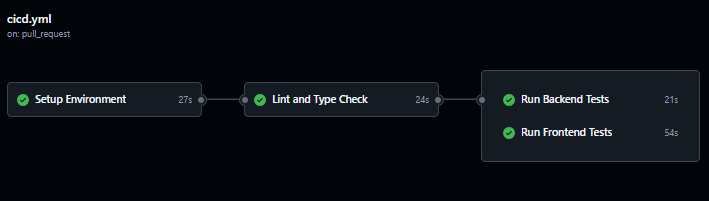
\includegraphics[scale=1.3]{../assets/Ci.png}
  \caption{CI/CD pipeline stages}
  \label{fig:survey6}
\end{figure}
\newpage
\section{Trace to Requirements}
\begin{table}[H]
  \centering
  \begin{tabular}{|c|c|}
  \hline
  \textbf{Unit Test ID} & \textbf{Requirement ID} \\ \hline
  UT-1          & NFR-LF1, NFR-OE2            \\ \hline
  UT-2          & FR1, FR7                    \\ \hline
  UT-3          & FR9                         \\ \hline
  UT-4          & FR1, FR2                    \\ \hline
  UT-5          & FR1, NFR-PR2                \\ \hline
  UT-6          & NFR-PR2                     \\ \hline
  UT-7          & FR3, FR11                   \\ \hline
  UT-8          & FR3, FR5, NFR-PR1, NFR-PR3  \\ \hline
  UT-9          & FR4, FR11                   \\ \hline
  UT-10         & FR4, NFR-PR1, NFR-PR3       \\ \hline
  UT-11         & NFR-SR1, NFR-LR1            \\ \hline
  UT-12         & NFR-SR1, NFR-LR1            \\ \hline
  UT-13         & NFR-LF1, NFR-LF2            \\ \hline
  UT-14         & NFR-UH1                     \\ \hline
  UT-15         & NFR-LF1, NFR-LF2            \\ \hline
  UT-16         & NFR-UH1                     \\ \hline
  UT-17         & FR8                         \\ \hline
  UT-18         & FR4                         \\ \hline
  UT-19         & NFR-UH1                     \\ \hline
  UT-20         & FR7                         \\ \hline
  UT-21         & FR6, NFR-PR1, NFR-HS2       \\ \hline
  UT-22         & FR6                         \\ \hline
  UT-23         & FR6, NFR-MS1                \\ \hline
  UT-24         & FR4                         \\ \hline
  UT-25         & FR4                         \\ \hline
  UT-26         & FR3, FR10, NFR-PR3          \\ \hline
  UT-27         & FR3, NFR-LR2                \\ \hline
  UT-28         & FR7                         \\ \hline
  UT-29         & FR2, FR7, FR9, NFR-MS1, NFR-LR2 \\ \hline
  UT-30         & FR2, FR7, FR9               \\ \hline
  UT-31         & FR1, NFR-SR1                \\ \hline
  UT-32         & FR1, FR7, NFR-SR1           \\ \hline
  \end{tabular}
  \caption{Trace from Unit Tests to Requirements  \citep{SRS}} 
  \label{tab:ut-req-trace}
  \end{table}

\section{Trace to Modules}
\begin{table}[H]
\centering
\begin{tabular}{|l|l|}
\hline
\textbf{Unit Test} & \textbf{Modules Tested} \\ \hline
UT-1 & M1, M2 \\ \hline
UT-2 & M1, M13, M14 \\ \hline
UT-3 & M13 \\ \hline
UT-4 & M1, M6 \\ \hline
UT-5 & M2 \\ \hline
UT-6 & M2 \\ \hline
UT-7 & M3, M12 \\ \hline
UT-8 & M3, M12 \\ \hline
UT-9 & M4, M11 \\ \hline
UT-10 & M4, M11 \\ \hline
UT-11 & M5 \\ \hline
UT-12 & M5 \\ \hline
UT-13 & M6 \\ \hline
UT-14 & M6 \\ \hline
UT-15 & M7 \\ \hline
UT-16 & M7 \\ \hline
UT-17 & M8 \\ \hline
UT-18 & M8 \\ \hline
UT-19 & M9 \\ \hline
UT-20 & M9 \\ \hline
UT-21 & M10 \\ \hline
UT-22 & M10 \\ \hline
UT-23 & M10 \\ \hline
UT-24 & M11 \\ \hline
UT-25 & M11 \\ \hline
UT-26 & M12 \\ \hline
UT-27 & M12 \\ \hline
UT-28 & M13 \\ \hline
UT-29 & M13 \\ \hline
UT-30 & M13 \\ \hline
UT-31 & M14 \\ \hline
UT-32 & M14 \\ \hline
\end{tabular}
\caption{Traceability Matrix: Unit Tests to Modules \citep{}}
\label{tab:traceability}
\end{table}
  
  \clearpage
  \newpage
\section{Code Coverage Metrics}
The following code Coverage analysis was obtained from the automated tests that were run on the \href{https://github.com/RezaJodeiri/CXR-Capstone/actions/runs/13778734218}{CI/CD pipeline}:
\begin{figure}[ht!]
  \centering
  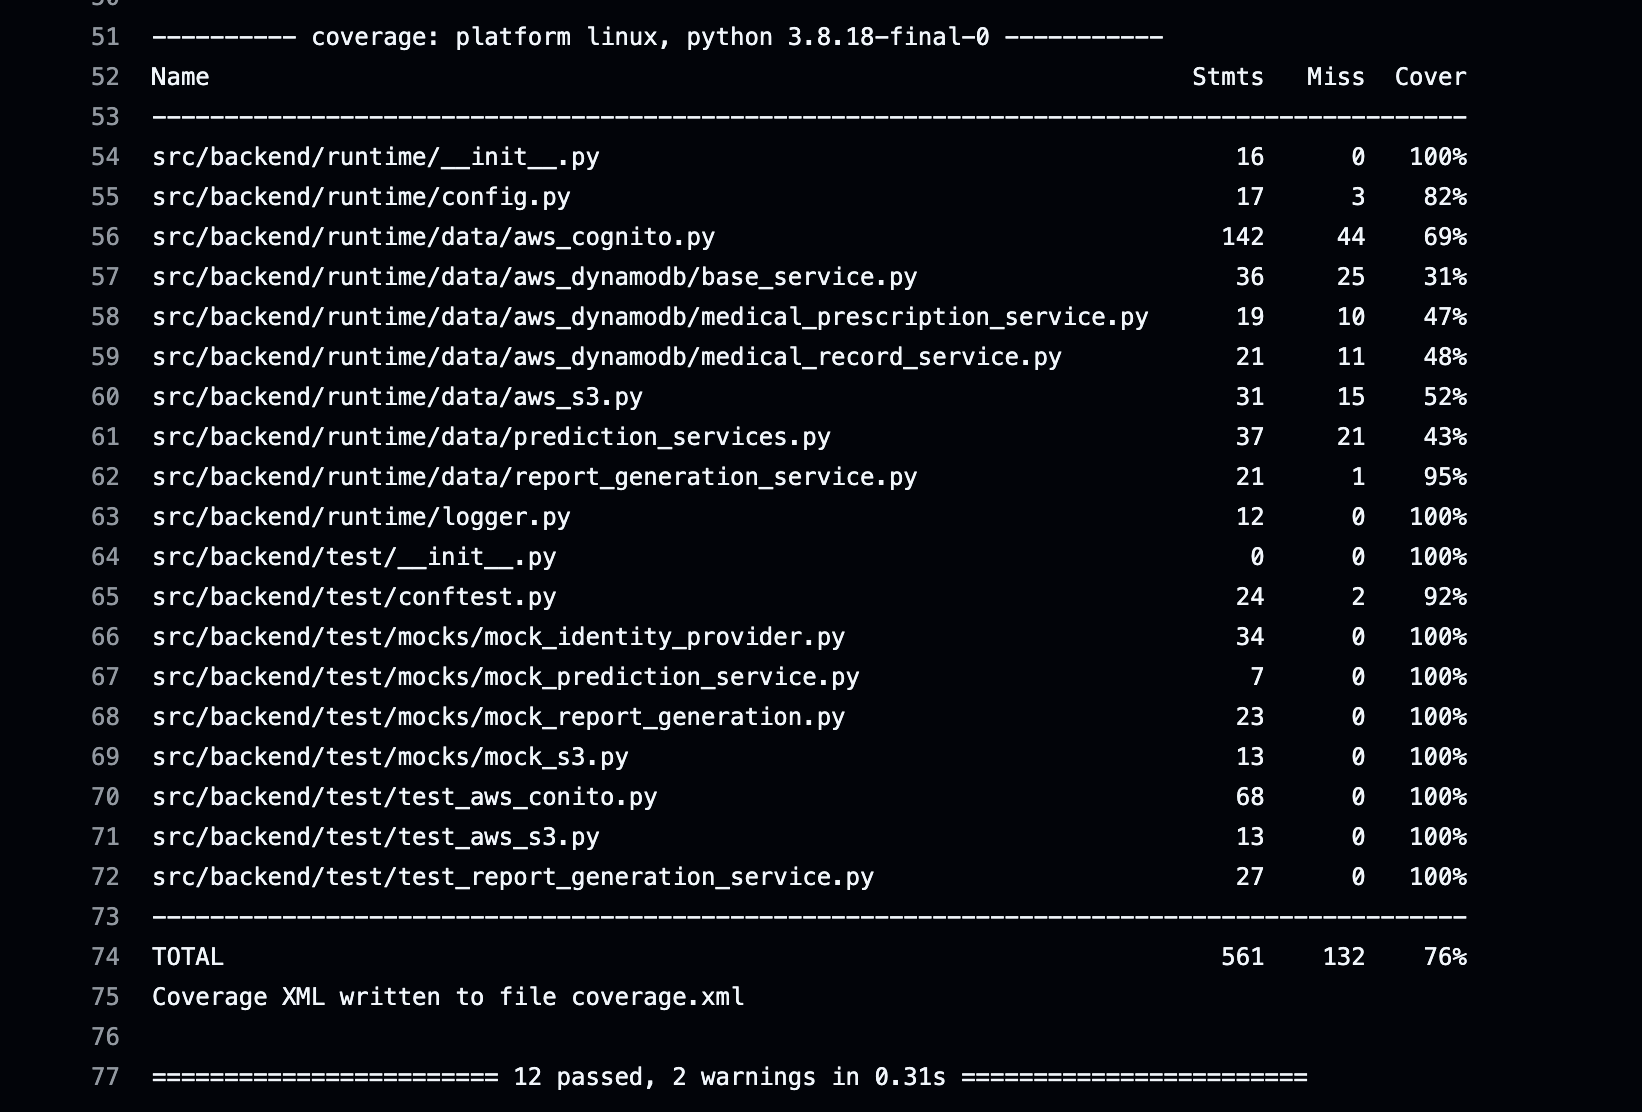
\includegraphics[scale=0.6]{../assets/cov.png}
  \caption{Code Coverage}
  \label{fig:Coverage}
\end{figure}

\vspace{10pt}
\noindent Our codebase achieved an overall test coverage of 76\% across 561 statements, with 132 statements not covered by our test suite. Several components demonstrate excellent test coverage, with 8 files reaching 100\% coverage, including core modules like the logger implementation and various test mocks. The report generation service also shows strong coverage at 95\%.

\vspace{10pt}
\noindent Areas requiring additional test attention are primarily in the AWS DynamoDB services layer, with the base service at 31\% coverage and medical-related services ranging from 43-52\%. These lower coverage percentages reflect the complexity of fully testing cloud service integrations in isolation. The AWS Cognito authentication module also presents opportunities for improvement at 69\% coverage.

\vspace{10pt}
\noindent It should be noted that several components with lower test coverage rates directly interact with third-party services such as AWS DynamoDB, AWS S3, AWS Cognito, and the OpenAI API. These integrations present unique testing challenges:

\begin{itemize}
    \item[-] External service calls require complex mocking frameworks to simulate responses
    \item[-] Some edge cases are difficult to reproduce without accessing the actual service
    \item[-] Authentication flows with services like Cognito involve multi-step processes that are challenging to test in isolation
    \item[-] API contracts may change with service updates, particularly with evolving services like OpenAI
\end{itemize}

\noindent While we have implemented mocks for these services in our testing environment, achieving complete coverage remains challenging without introducing tests that may provide false confidence. Our testing strategy prioritizes reliable validation of core business logic while acknowledging the inherent limitations in testing third-party integrations.
\vspace{10pt}

\noindent Additionally, our frontend testing suite achieved comprehensive coverage across React components and utilities, with particular focus on critical user interface elements. The tests were implemented using Jest and React Testing Library.The following were the frontend tets that we perforemd:
\begin{figure}[ht!]
  \centering
  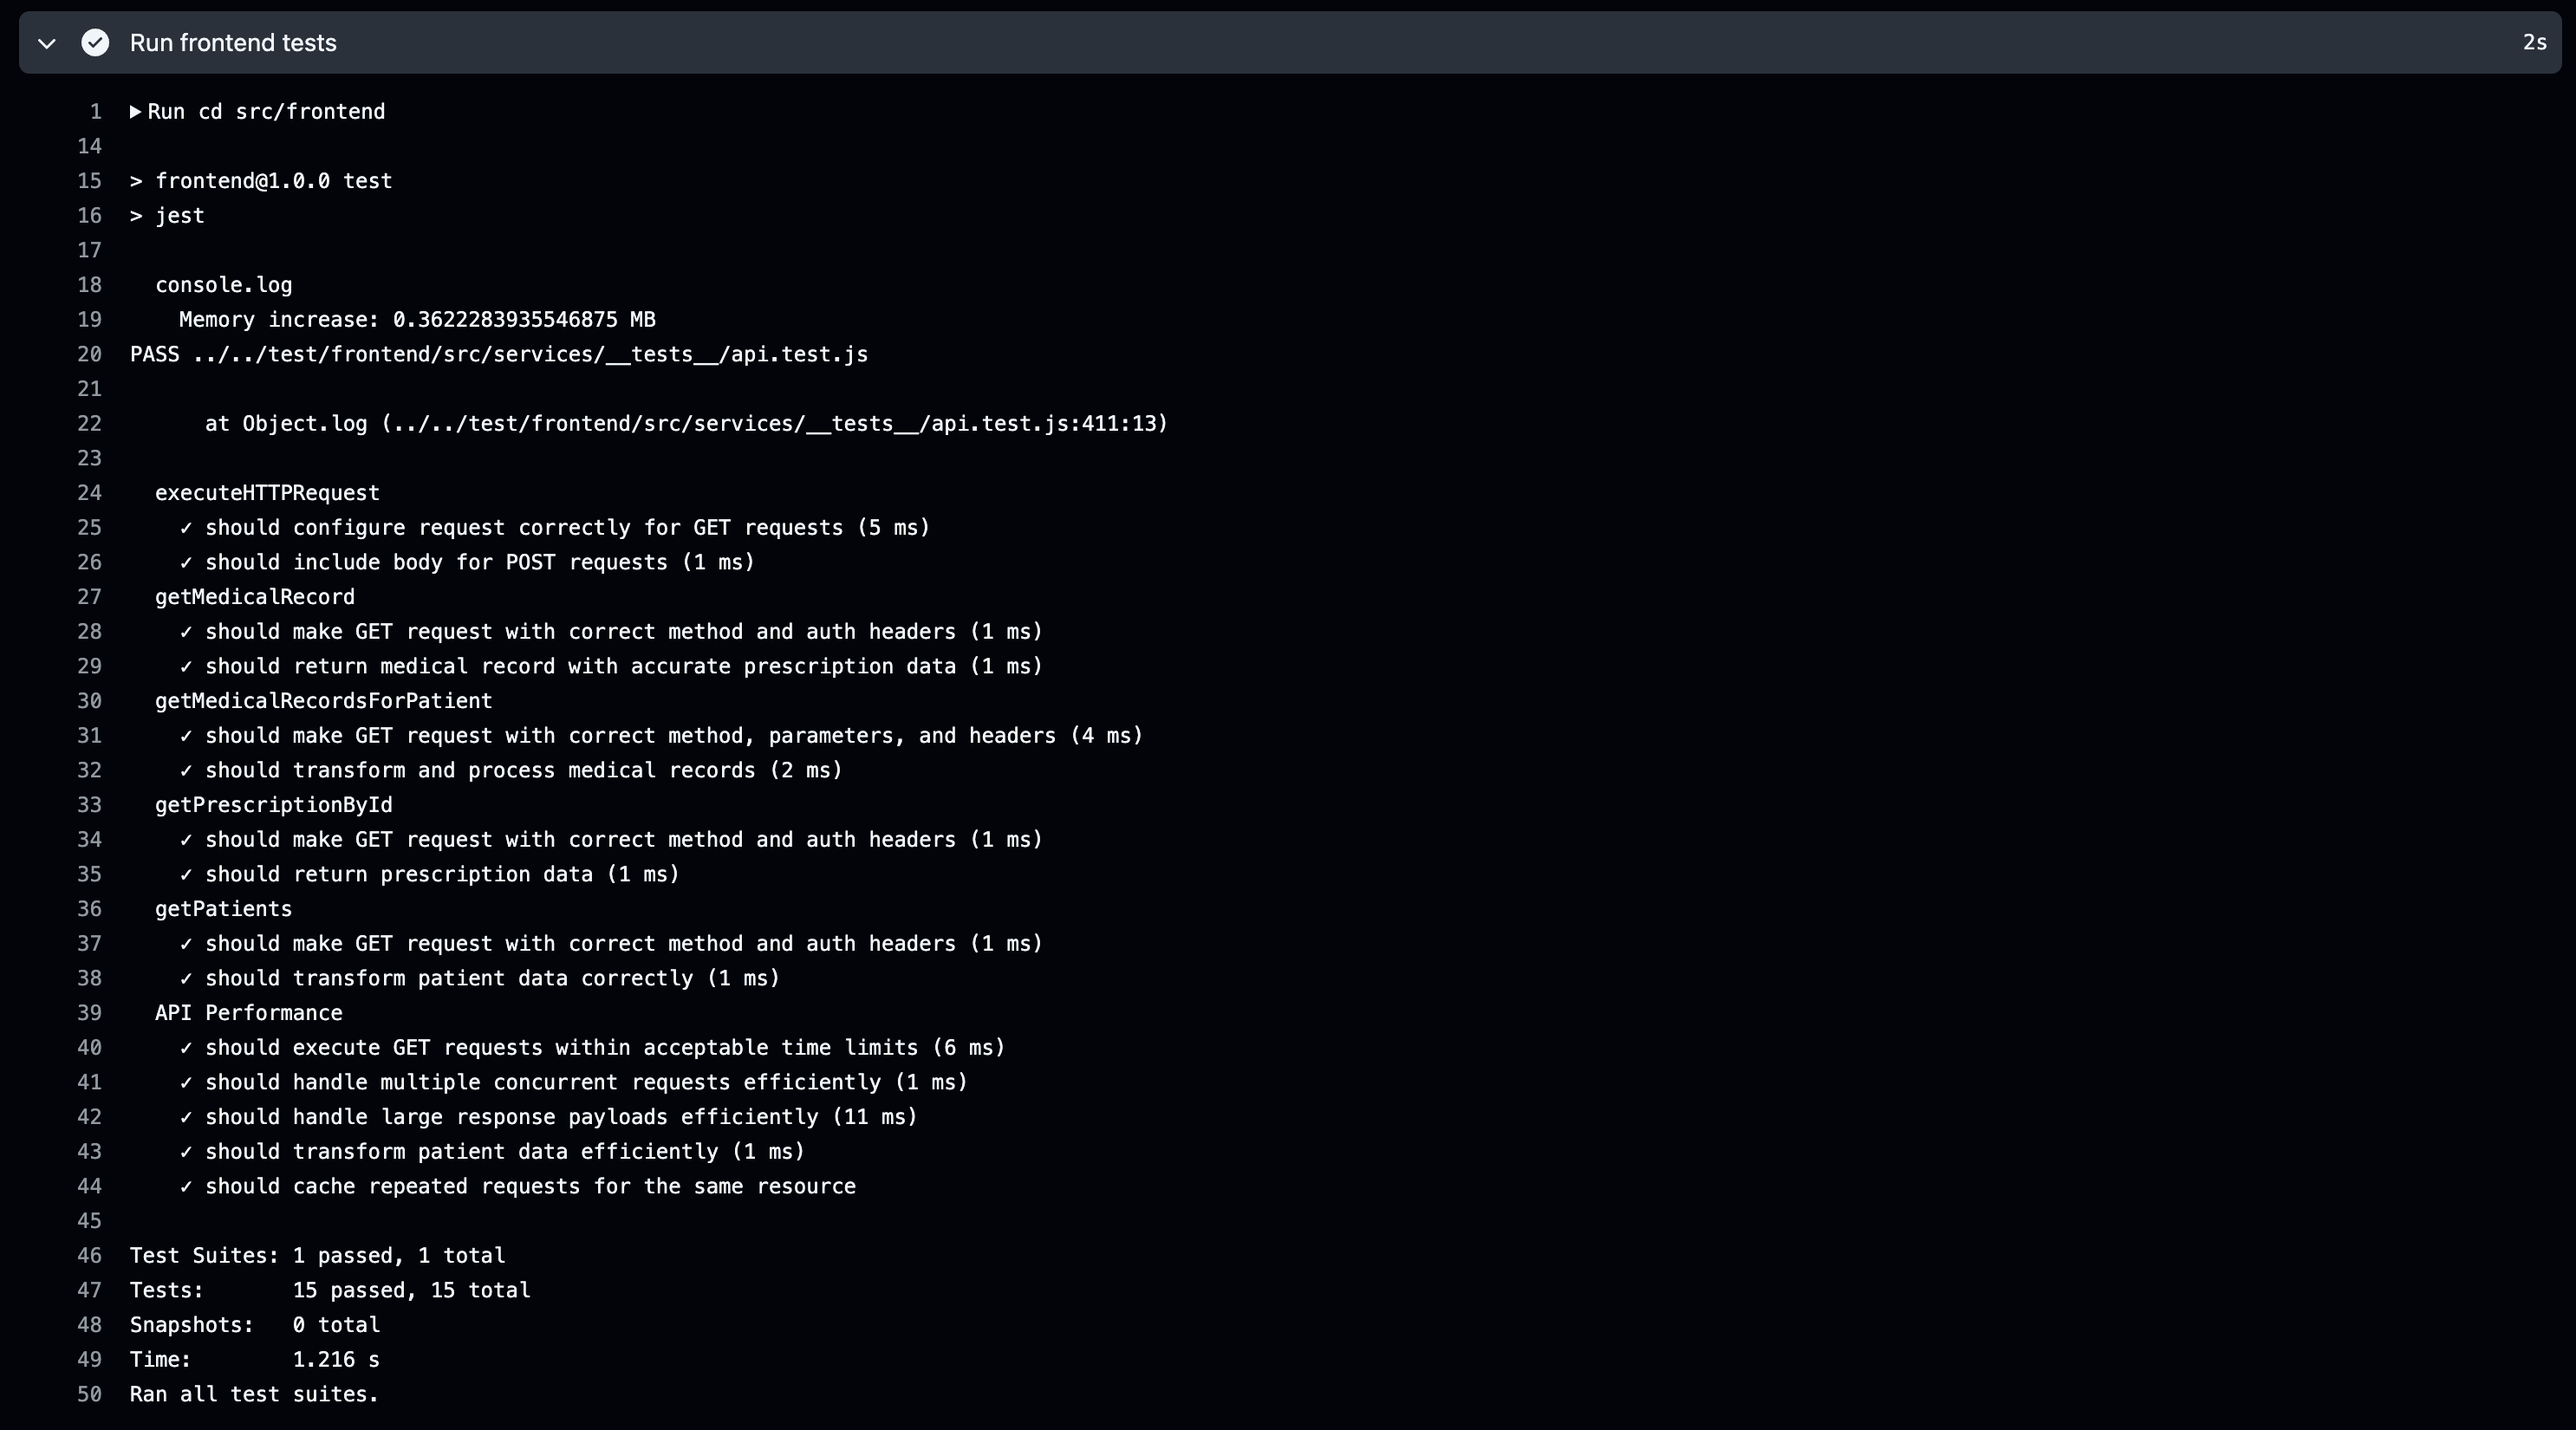
\includegraphics[scale=0.35]{../assets/front.png}
  \caption{Frontend Tests}
  \label{fig:Coverage}
\end{figure}

\newpage
\bibliographystyle{plainnat}
\bibliography{../../refs/References}



\newpage{}
\section*{Appendix --- Reflection}
  \textbf{What went well while writing this deliverable?} \\\\
  The modular design of our system allowed us to create clear and well-structured unit tests. Each test targeted its own specific business logic and did not interfere with others, which helped us achieve more comprehensive unit test coverage. By following SOLID principles and maintaining a clear separation of concerns, we designed precise and maintainable tests that effectively targeted individual components. This modular approach enabled us to create highly focused test cases, minimizing dependencies and improving fault isolation. Leveraging mock services and data allowed us to systematically verify each component and separate concerns, ensuring that each module functioned correctly in isolation with its expected functionalities. Additionally, these tests were seamlessly integrated into our CI/CD pipeline, enabling automated validation at every stage of development. This approach streamlined the testing process and also improved reliability by allowing us to simulate various scenarios and edge cases, ensuring consistent performance across deployments.
  \newline \newline \textbf{What pain points did you experience during this deliverable, and how did you resolve them?} \\\\
  One major challenge was handling unexpected deviations from the VnV Plan. Some tests and validation activities required adjustments because real-world implementation differed from our initial assumptions. To address this, we removed certain tests and modified others to better fit the project scope. Another challenge we faced was testing non-functional requirements (NFRs), particularly in gathering sufficient feedback from qualified testers. To address this, our team implemented an external testing approach using a Google Form to collect responses. However, we encountered difficulties in obtaining an adequate number of responses from eligible testers, such as medical professionals as our project was not in a collaboration with hospitals / medical services. The limited participation made it challenging to thoroughly validate certain NFRs, such as usability and performance in real-world scenarios. Additionally, creating unit tests for the code was a significant task. However, by effectively distributing the workload among team members, we successfully developed and passed all necessary tests.
  \newline  \newline \textbf{Which parts of this document stemmed from speaking to your client(s) or a proxy (e.g., your peers)? Which ones were not, and why?}  \\\\
  Some aspects of this document stemmed from discussions with our proxies (peers), particularly regarding non-functional requirements testing as some of them couldn't be tested directly via unit tests. (usability, user experience, and looks and feels). While unit tests focus on validating specific functions in isolation, they do not capture real-world interactions, user satisfaction, or how well the system meets stakeholder expectations. Surveys allowed us to gather qualitative and quantitative feedback from relevant users, helping us assess aspects like ease of use, efficiency, and overall satisfaction. Our unit tests were primarily designed to validate the correctness, reliability, and functionality of individual components in isolation. They focused on ensuring that each module adhered to its expected behavior based on predefined business logic, rather than incorporating input from peers or end-users.
  \newline
  However, not all sections were based on client input. Technical implementation details, such as internal testing methodologies and the choice of specific testing frameworks, were determined by the development team. This distinction exists because clients typically focus on high-level functionality and usability, while the development team makes technical decisions regarding implementation and testing strategies. \\ 
  \newline
  \textbf{In what ways was the Verification and Validation (VnV) Plan different from the activities that were actually conducted for VnV?}
  \vspace{-10pt}
\subsubsection*{Differences Between the VnV Plan and VnV Report}
  \begin{itemize}
  \item[-] In the VnV Plan, we initially outlined the testing for functional and non-functional requirements. However, the project was not fully mature and due to this the VnV Report had to be adjusted to reflect the actual testing conducted. This was shown to be evident through the removal of NFRs and FRs while new ones being added.  
  \item[-] The original VnV Plan assumed static test data for validation, but as development progressed, we realized that model performance varied significantly across different datasets. The VnV Report reflects additional real-world test cases added to evaluate model robustness across various demographic and clinical conditions. This was also later changed in the VNV plan to match.
  \item[-] Initially planned as a basic text output, this feature was expanded in the VnV Report to include structured templates for easier clinical use.
  \end{itemize}
  
\subsubsection*{Reasons for Deviations}
  \noindent These deviations were necessary due to:
  \begin{itemize}
  \item[-] Technical constraints, particularly in model interpretability and performance generalization.
  \item[-] Regulatory considerations, requiring expanded fairness and bias assessments beyond the original scope.
  \item[-] Stakeholder feedback, which emphasized the need for more real-world validation scenarios. By doctors and radiologist to test the system and what they would want to see in our application.
  \item[-] Resource limitations which led to adjustments in testing priorities and methodologies.
  \end{itemize}
  
\subsubsection*{Lessons Learned for Future VnV Planning}
  \noindent While deviations were unavoidable, they provided valuable insights for improving future VnV planning. To better anticipate such changes, our team could:
  \begin{itemize}
    \item[-] Planning during the early maturity of the project is difficult and should be revisited as the project matures.
    \item[-] Early real-world testing is critical – testing only on predefined datasets missed real-world challenges, such as low-quality scans.
    \item[-] Explainability should be prioritized from the start – assuming simple feature visualization was sufficient led to delays in meeting doctor expectations.
    \item[-] Load testing should be iterative – scalability concerns were only identified late in development, making fixes more complex.
    \item[-] Stakeholder feedback must be integrated earlier – doctors provided critical usability insights only after testing, when design changes were harder to implement.
    \end{itemize}

\subsection*{Conclusion}
  In conclusion, the Verification and Validation process for our project has been a comprehensive and iterative journey. We have successfully evaluated both functional and non-functional requirements, ensuring that our system meets the high standards expected in a clinical setting by removing unnecessary requirements and adding new ones. The deviations from the original VnV Plan aided to address our challenges, technical constraints, and stakeholder feedback. These adjustments have refined our system, making it more robust, user-friendly, and aligned with regulatory requirements.
  \noindent The lessons learned from this process highlight the importance of early and continuous testing, stakeholder engagement, and flexibility in planning. By incorporating these insights into future projects, we can improve our VnV strategies and deliver even more reliable and effective solutions.
  \noindent Hence, the VnV activities have validated the performance, usability, and security of our system, providing confidence in its readiness for deployment in real-world healthcare environments.

  \newpage
  \section*{Appendix A --- Survey Results (NFR quality 1)}\label{appendix:A}
  
  \begin{figure}[ht!] 
    \centering
    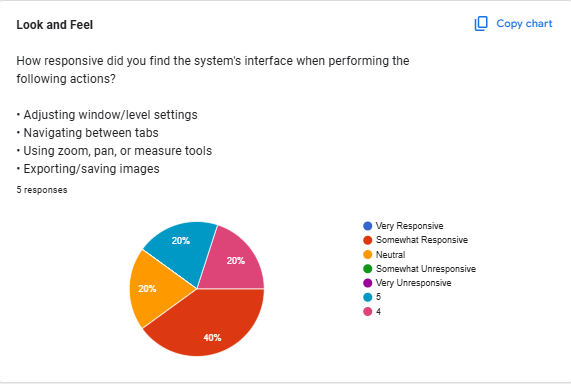
\includegraphics[scale=1.3]{../assets/s1.png}
    \caption{Survey results for Question 1}
    \label{fig:survey1}
  \end{figure}
  
  \begin{figure}[ht!]
    \centering
    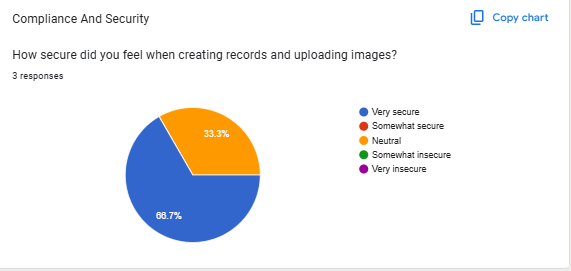
\includegraphics[scale=1.3]{../assets/s2.png}
    \caption{Survey results for Question 2}
    \label{fig:survey2}
  \end{figure}
  
  \begin{figure}[ht!]
    \centering
    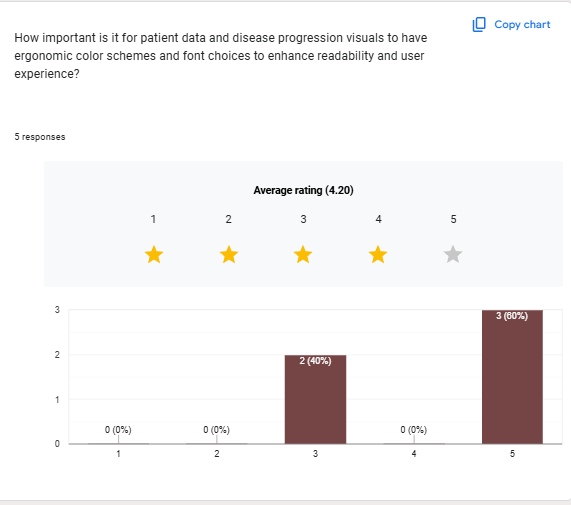
\includegraphics[scale=1.1]{../assets/s3.png}
    \caption{Survey results for Question 3}
    \label{fig:survey3}
  \end{figure}
  \begin{figure}[ht!]
    \centering
    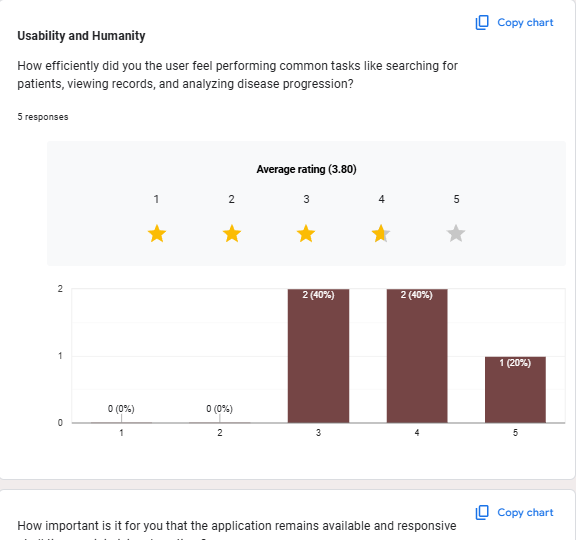
\includegraphics[scale=1.1]{../assets/s4.png}
    \caption{Survey results for Question 4}
    \label{fig:survey4}
  \end{figure}
  
  \begin{figure}[ht!]
    \centering
    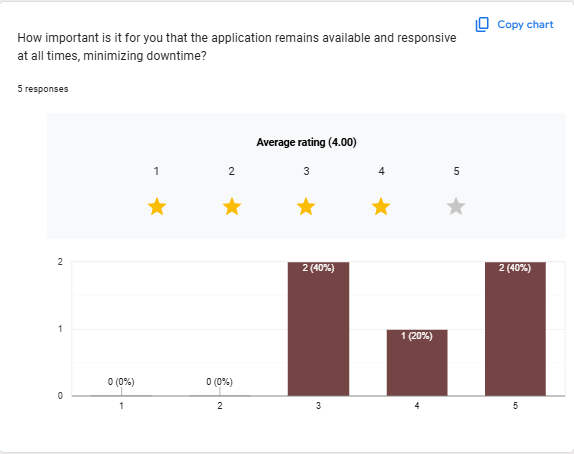
\includegraphics[scale=1.1]{../assets/s5.png}
    \caption{Survey results for Question 5}
    \label{fig:survey5}
  \end{figure}
  
  \begin{figure}[ht!]
    \centering
    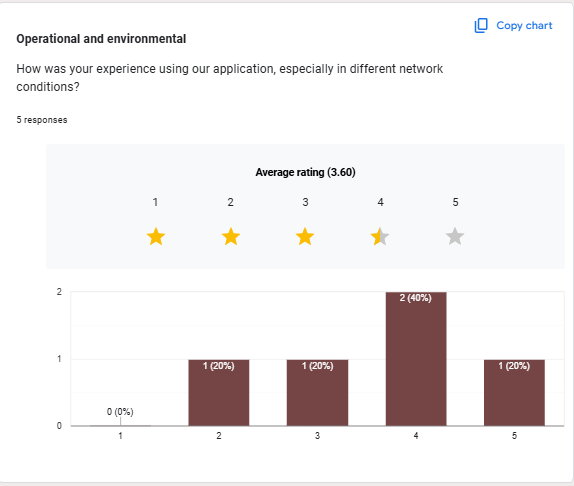
\includegraphics[scale=1.1]{../assets/s6.png}
    \caption{Survey results for Question 6}
    \label{fig:survey6}
  \end{figure}
  
  \begin{figure}[ht!]
    \centering
    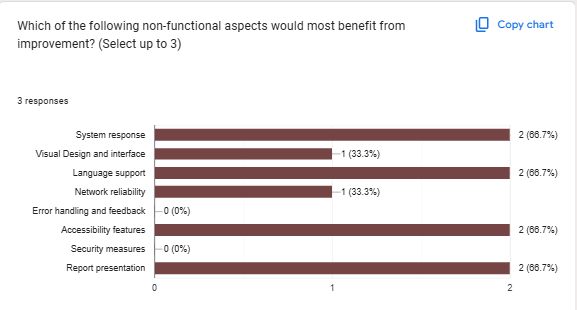
\includegraphics[scale=1.5]{../assets/s7.png}
    \caption{Survey results for Question 7}
    \label{fig:survey7}
  \end{figure}
  
  \begin{figure}[ht!]
    \centering
    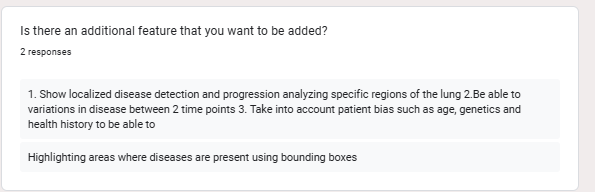
\includegraphics[scale=1.5]{../assets/s8.png}
    \caption{Survey results for Question 8}
    \label{fig:survey8}
  \end{figure}

\clearpage

\section*{Appendix B --- Performance Test (NFR quality 2)}\label{appendix:B}
\begin{figure}[ht!]
  \centering
  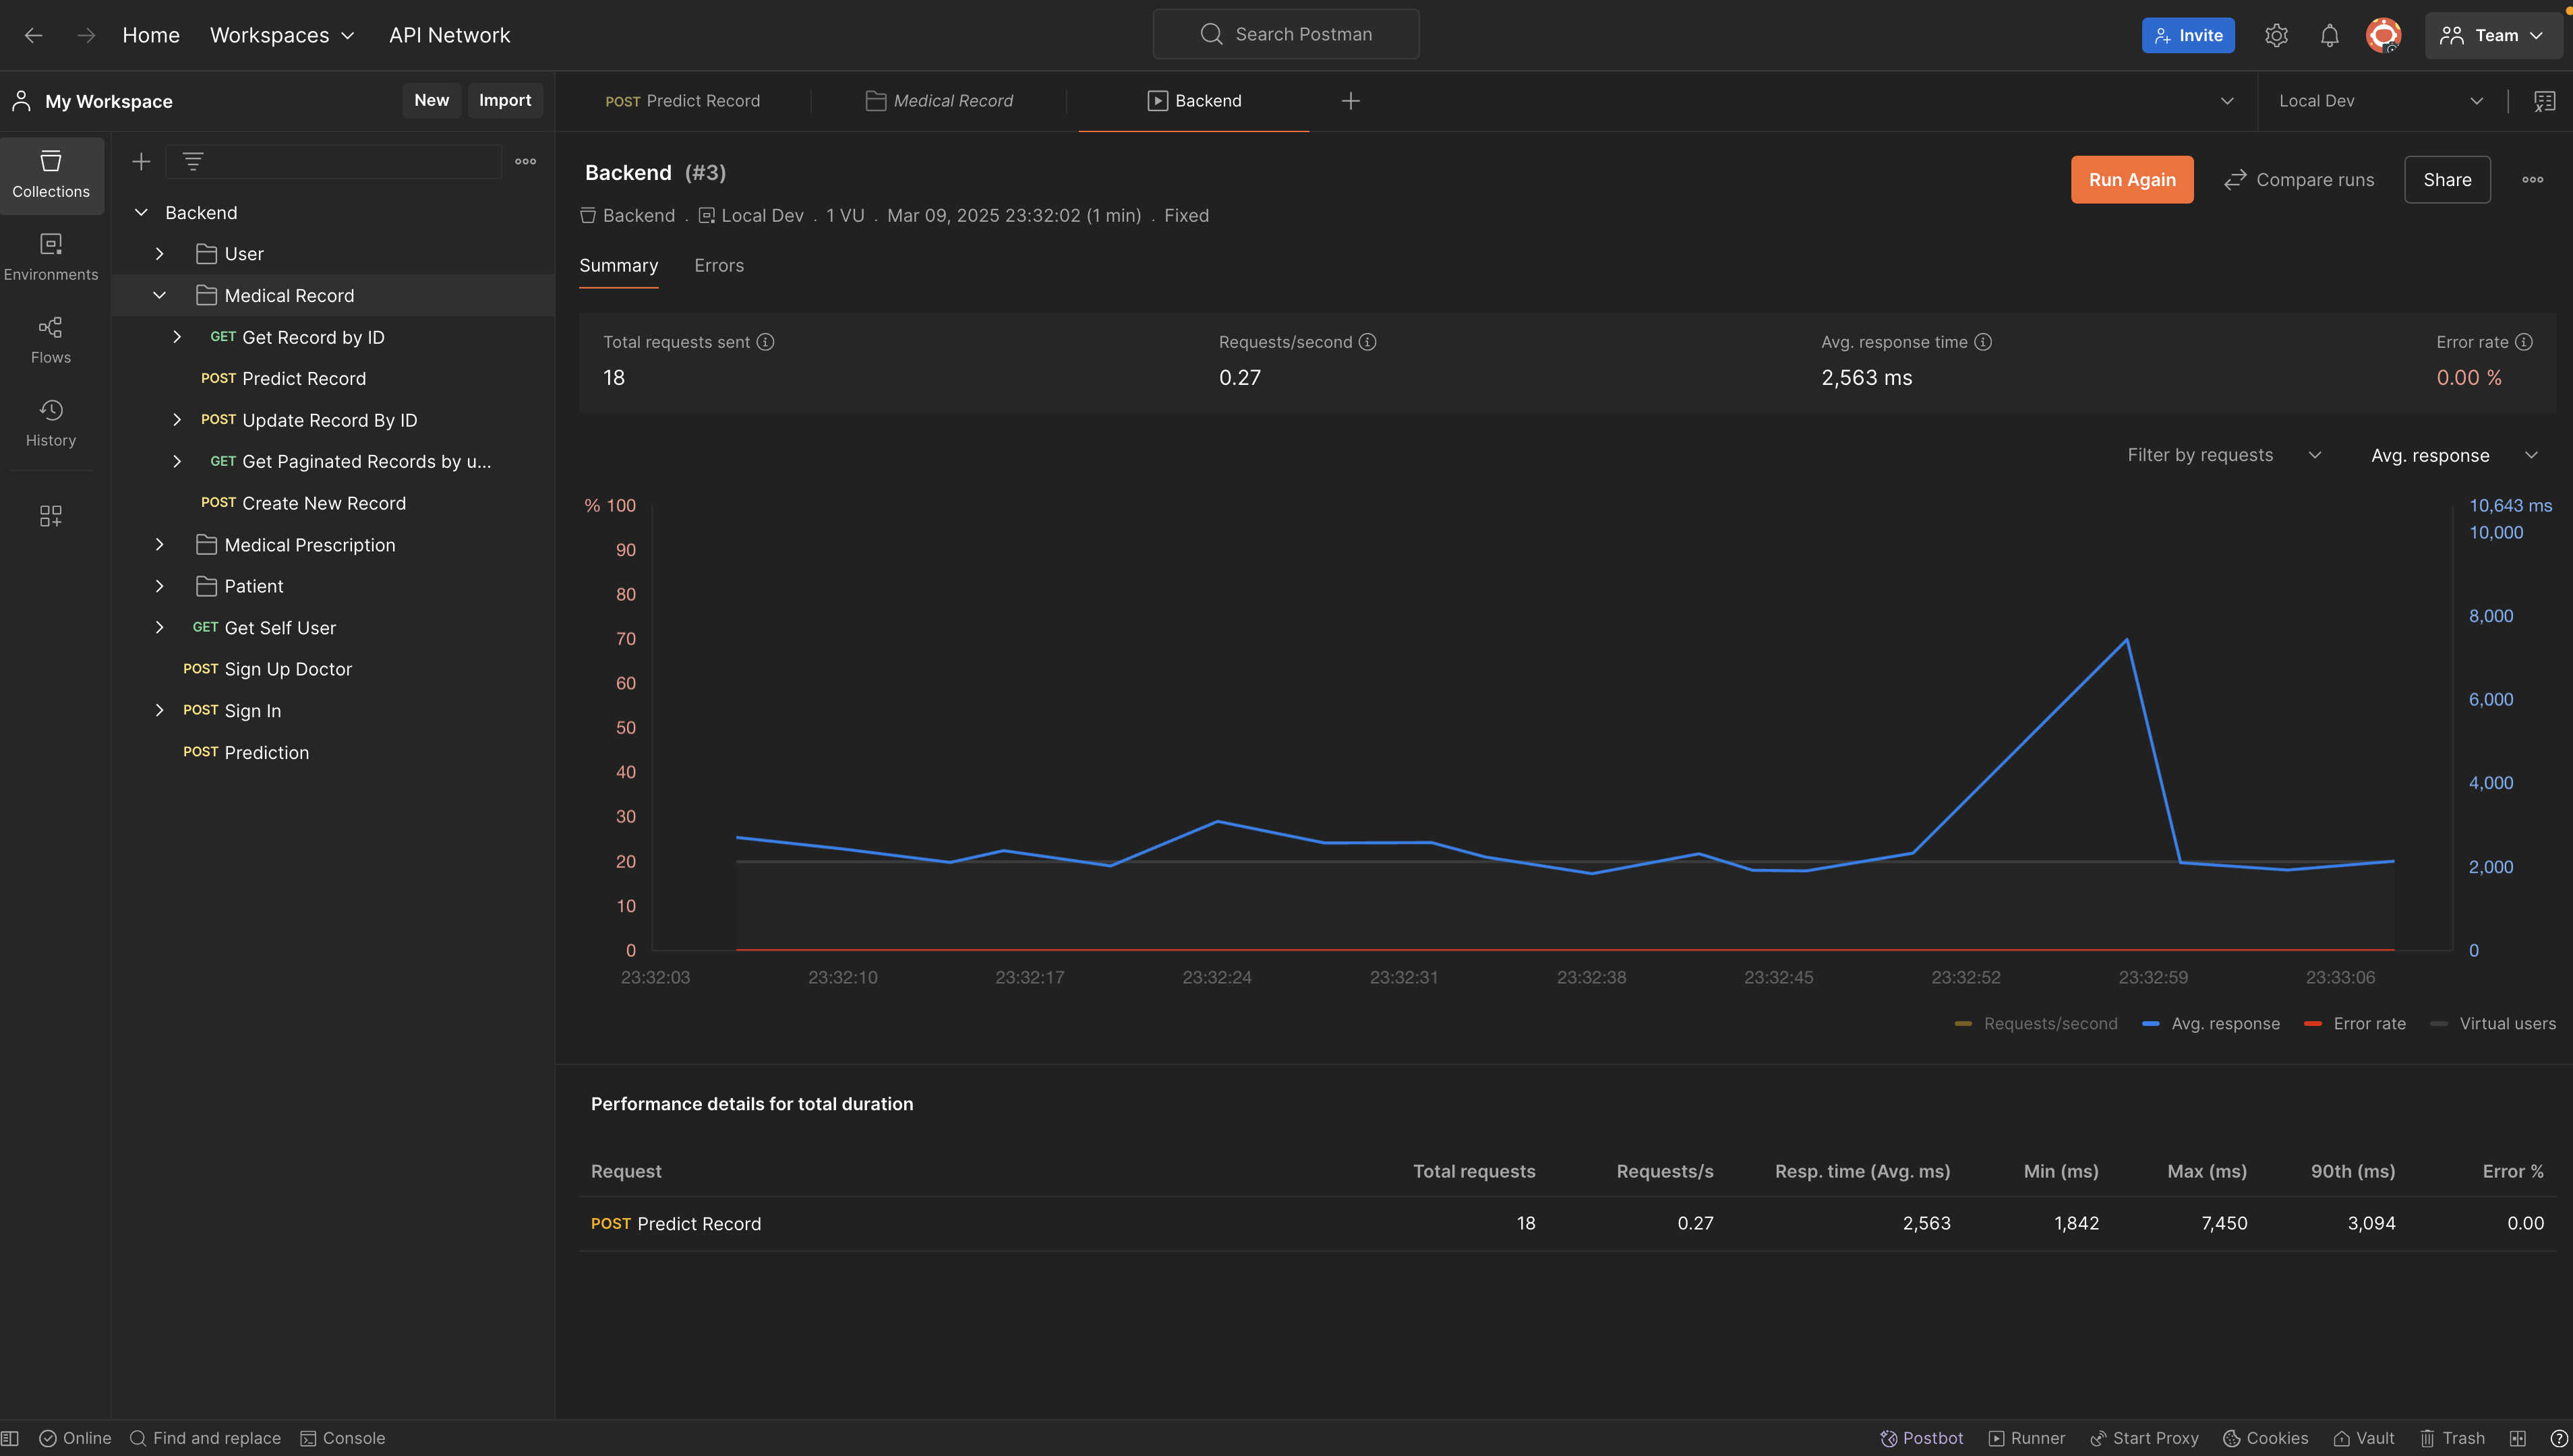
\includegraphics[scale=0.24]{../assets/Perf.png}
  \caption{Survey results for Question 8}
  \label{fig:survey8}
\end{figure}

\begin{figure}[ht!]
  \centering
  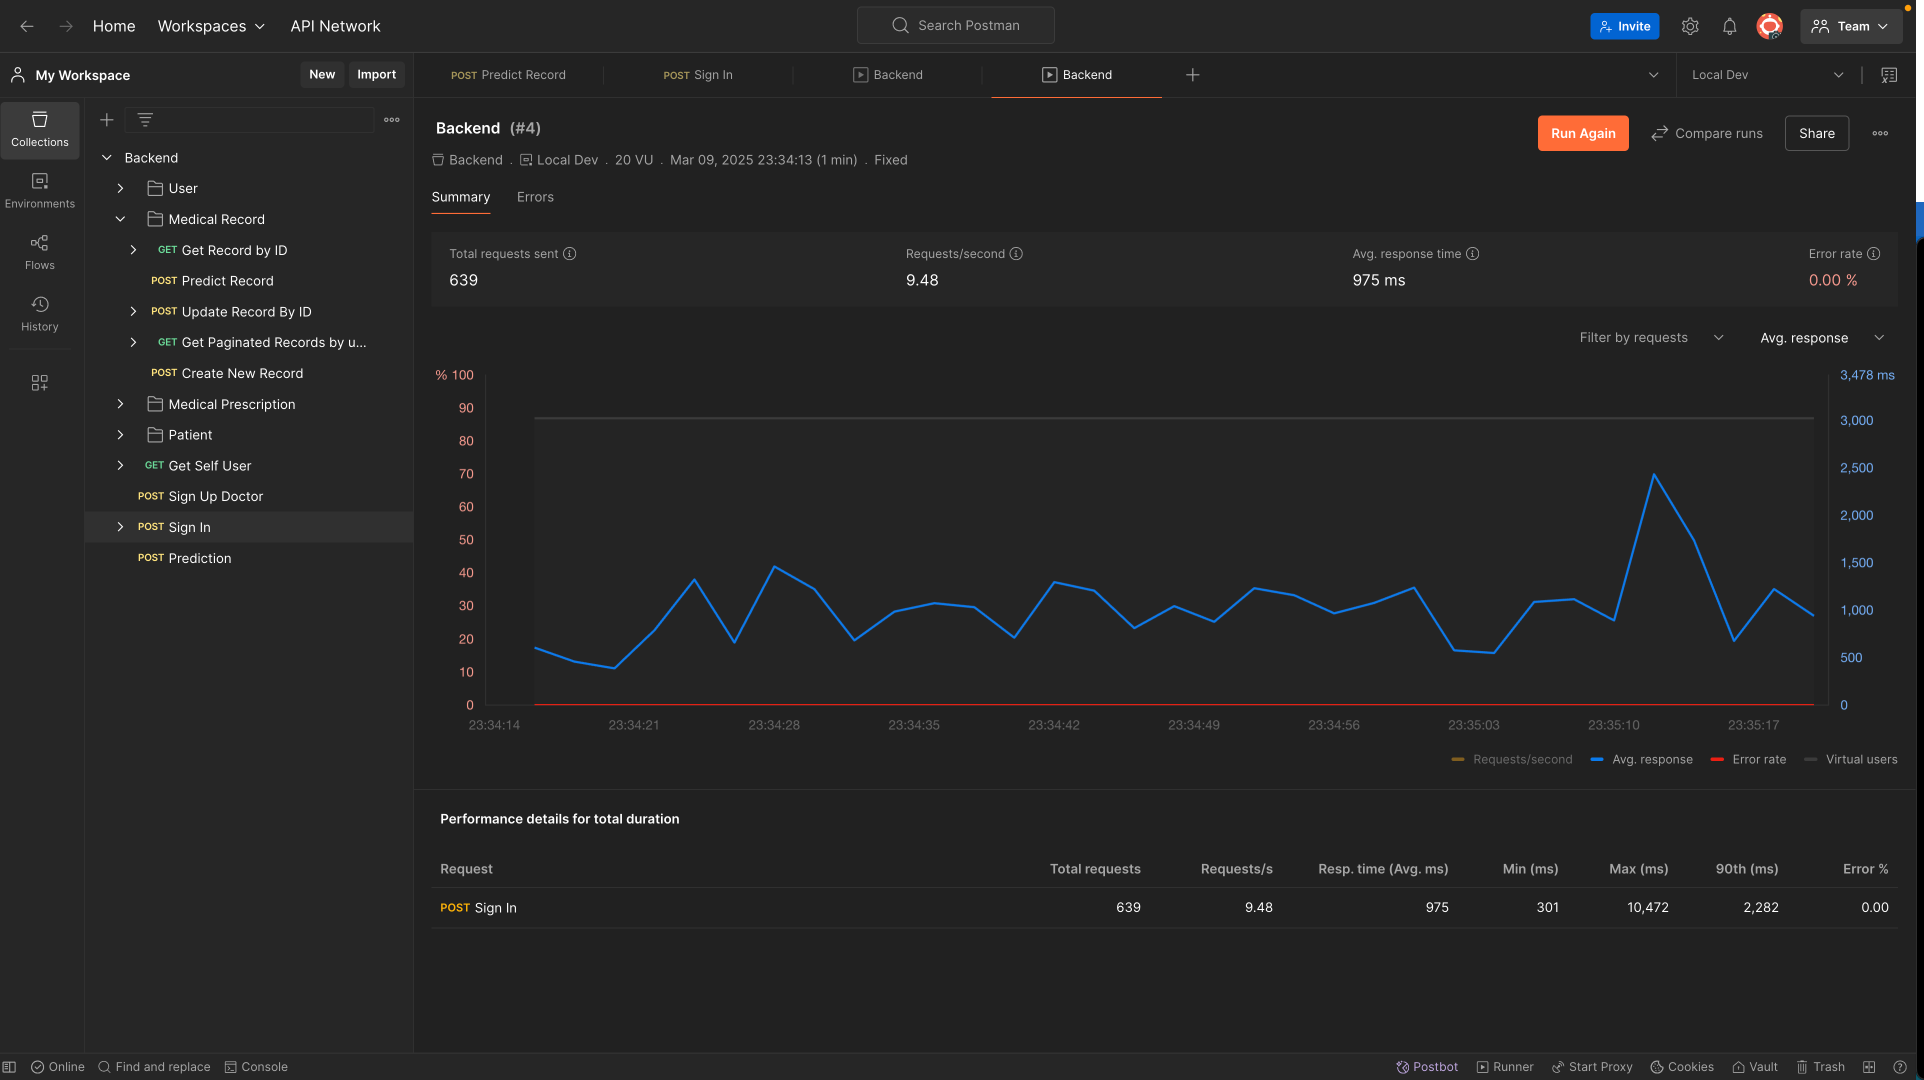
\includegraphics[scale=0.47]{../assets/Perf2.png}
  \caption{Survey results for Question 8}
  \label{fig:survey8}
\end{figure}
\end{document}